\documentclass[12pt, oneside]{extbook} % the document type needs to be change
\usepackage{geometry}
\usepackage{listings}
\usepackage{graphicx}

\geometry{
	a4paper,
	left = 1.5 cm,
	right = 1.5 cm,
	top = 2cm,
}

\title{Network and System Defense}

\begin{document}
\maketitle
\tableofcontents
\newpage
\part{Parte Hardware}
\chapter{Introduzione}
In cybersecurity, ci sono almeno 5 aree esterne differenti che si mischiano fra loro, e poi 3 aree interne relative all'hardware ed al software.\\ "L'attore principale" sono applicazioni Internet-based:
\begin{itemize}
\item vulnerabilità del sistema, della rete etc
\item come difendersi o evitare tali vulnerabilità, o almeno mitigarle
\end{itemize}
Molta configurazione pratica: laboratori da 0, ma è utile rifare tutto a casa (\textbf{CAZZI}).\\ Per via del fatto che è davvero difficile oggi separare cosa è la rete da cosa è il software, è utile parlare di tutti i diversi campi che riguardano sia la rete che il software.\\ Punti chiave:
\begin{itemize}
\item Access networks and perimetral security: Ethernet, VLAN, IPv6, 802.11x, firewall, packet classification algorithms
\item Core networks: BGP, MPLS, DDos e Botnets, VPNs con BGP
\item End to End security: PKIs, DNS security, HTTPS, Overlay VPNs
\item Sw and Operating System
\item Virtualization \& Cloud 
\end{itemize}
Piattaforme da utilizzare per la parte da 6 CFU (Hardware):
\begin{itemize}
\item GNS3
\item Tinycore Linux
\item VMware o Virtual Box: Virtual Box sembra lavorare meglio con GNS3
\item Cumulus Linux: serve per emulare le funzionalità di livello 2 di uno switch. Net OS, \textbf{scaricare la versione 4.1} e non le ultime. C'è un insieme di VM pronte per essere installate su un virtualizzatore
\item Immagini CISCO (da cercare online, if you know what I mean)
\item Lubuntu
\item Ubuntu server
\end{itemize}
\chapter{Introduzione alla cybersecurity}
Ci sono 3 fattori principali quando si parla di cyberscurity:
\begin{itemize}
\item Cosa bisogna proteggere?
\item Da quali minacce? Ci sono diverse fonti di attacco da cui proteggersi
\item Come fare per contrastare queste minacce? Integrità, encryption, etc...
\end{itemize}
\paragraph{Definizione di computer security:}le misure ed i controlli che garantiscono confidenzialità, integrità e disponibilità degli assets dei sistemi informativi, incluso hardware, software etc...
\begin{itemize}
\item confidenzialità: i dati sono privati, le informazioni confidenziali non sono note ad entità non autorizzate. Esempi: usare SSH o HTTPS per scambiare credenziali con un server.
\item Privacy: (slides)
\item Integrità: se dei dati, indica che essi sono cambiati solo in maniera autorizzata. Se voglio traferire un messaggio con cui trasferisco del denaro, non voglio che il contenuto sia compromesso. Se si parla di integrità dei sistemi, si intende che il sistema performi come deve (vedi slides)
\item disponibilità: si assicura che il sistema lavori in maniera corretta e che i servizi non siano negati ad utenti autorizzati
\end{itemize}
Altri aspetti importanti:
\begin{itemize}
\item Authenticity: dell'utente, indica che sia possibile verificare che l'utente è chi dice di essere. Della sorgente: capacità di verificare che un messaggio arriva da una sorgente effettivamente affidabile.
\item altri ... (slides)
\end{itemize} 
\textbf{ALTRE IMPORTANTI DEFINIZIONI CHE SI TROVANO SULLE SLIDES}. \\ Quali sono le diverse superfici di attacco:
\begin{enumerate}
\item la rete stessa: i sistemi sono Internet-based, quindi è sempre possibile attaccare la rete. Attaccare la rete implica sfruttare vulnerabilità della rete Internet: ARP, WEP, link fisici, intrusioni nella rete etc...
\item attacchi al software: vulnerabilità nell OS, server web, code injection etc...
\item attacchi all'umano: molte vulnerabilità create da noi stessi, social engineering, errori umani, mancanza di competenze etc...
\end{enumerate}
È importante non pensare che la sicurezza sia data solo dalla tecnologia, ma anche dalle persone.\\ \paragraph{CIS critical security controls:} 20 applicazioni pratiche che la SANS suggerisce di applicare per verificare la sicurezza di una corporation (anche piccola Enterprise). Ogni controllo ha dei sotto-controlli più "concreti"\\ Quindi, non avendo il tempo di fare tutto, ci concentrare su alcuni aspetti fondamentali di tutto l'insieme visto.
\section{Lezione 2: vulnerabilità intrinseche IP/TCP}
Prima di capire le vulnerabilità, è necessaria una revisione dei protocolli di rete.
\subsection{Architettura di IP}
Intenet non è altro che una inter-connessione di reti che possono avere differenti tecnologie.\\ La comunicazione fra i device è possibile con IP, che è implementato sui livelli 1 e 2 (che sono indipendenti). Ogni dispositivo è identificato dall'indirizzo univoco a 32/64 bit (che seguono la nomenclatura CIDR), le diverse sotto-reti comunicano tramite i router ovvero un device IP che ha almeno 3 livelli dello stack Internet. Ha diverse interfacce che possono essere in diverse tecnologie: ADSL, Ethernet, Fibra etc...\\ Le operazioni compiute dai router:
\begin{itemize}
\item IP forwarding: longest prefix mathcing, manda un pacchetto verso la prossima interfaccia del percorso di rete. È diretta se la destinazione è nella subnet, mentre indiretta se serve trovare il next hop, quindi andare fuori dalla propria sotto-rete. Il next hop è un dispositivo nella propria sotto-rete che sa come arrivare alla destinazione.
\end{itemize}
Il goal di IP è quello di mandare il pacchetto a destinazione, l'Internet è diviso in Autonomous Systems all'interno dei quali si può configurare il routing come si vuole. Ma poi, serve scambiare informazioni fra As, si parla quindi di protocolli intra-AS come OSPF, RIP e protocolli inter-AS, come BGP.\\ C'è l'header per ogni pacchetto che ha i diversi campi (TTL, src, dest, protocol, checksum etc...), diverso fra IPv4 ed IPv6, differenze fra i due:
\begin{itemize}
\item header più piccolo in IPv6
\item no fragmentation in IPv6
\end{itemize}
\paragraph{Routing table:}struttura dati che associa una destinazione ad un next hop. Per il routing si usa il longest prefix matching, l'IP più "specifico" è quello scelto. La differenza principale fra host e router è che se un host riceve un pacchetto da una src non fra quelle locali, lo scarta; un router lo forwarda. Il forwarding standard basico è fatto in base all'indirizzo di destinazione. Dopo l'estrazione del pacchetto IP, se l'IP dest è locale, lo manda al livello superiore, altrimenti lo guarda nella tabella di routing: se non si trova un matching, il pacchetto è scartato. Altrimenti: se c'è un next hop, bisogna scoprire chi è, altrimenti basta scoprire il MAC associato all'IP.\\ La maggior parte dei pacchetti che vengono mandati vanno fuori dall'AS con cui si firma il contratto: possono esserci diversi AS di transito prima di arrivare al data center del sito a cui si cerca di connettersi.
\subsection{Vulnerabilità di TCP/IP}
Per design, IP e TCP non si preoccupano della sicurezza in quanto sono stati progettati quando la sicurezza non era un problema. C'è un certo numero di vulnerabilità intrinseche nei protocolli, ed è ancora così in quanto sono stati progettati senza pensare all'aspetto di sicurezza:
\begin{itemize}
\item Identification: i device della rete possono essere falsificati, è possibile spoofare l'IP address per dire di essere , ad esempio, un certo server web. Sia per i pacchetti generati dall'utente che per quelli forwardati. Se mandiamo un pacchetto di un legittimo server DNS, stiamo impersonificando il server stesso. Non ci sono meccanismi in IP per verificare l'autenticità di chi manda il pacchetto
\item Reputation: come è possibile verificare che l'origine del pacchetto è effettivamente la sorgente?
\item Confidentiality: non vogliamo che le informazioni scambiate sulla rete siano viste da 3e parti. Vorrei che solo il server veda i dati in uno scambio client-server. Ma intercettare il pacchetto in maniera "malevola" è fattibile ed anche decodificarlo perché l'header e l'IP sono in chiaro.\\ Il problema non è nella rete interna, ma passa per diversi AS (noi ci fidiamo solo del nostro): anche se il path fra sorgente e destinazione è fidato, è possibile fare hijaking su BGP, fra gli attacchi più pericolosi e in voga.
\item Integrity: voglio essere sicuro che il pacchetto non sia modificato durante il percorso fra src e dest. C'è il checksum, ma è calcolato su dati in chiaro, quindi non va bene come "codice" per poter assicurare l'integrità
\item Packet replication: non c'è sequence number nell'IP header nella sessione, non ci sono meccanismi per proteggersi da questo threat
\end{itemize}
\subsubsection{Dynamic mapping}
Le cose si complicano perché i protocolli Internet usano diversi meccanismi per implementare il mapping: ad esempio il DSN, ARP, 802.3 bridging (lo switch impara in automatico quale MAC è dietro quale porta) e questo è dinamico in quanto può cambiare nel tempo. Questo problema è presente in ogni layer ed anche questi meccanismi non sono stati penasti per essere sicuri.
\paragraph{DNS spoofing:}possiamo spoofare una richiesta DNS, quindi fare un hijack della sessione. Attacco triviale (e vecchio):
\begin{itemize}
\item sfruttiamo il mapping MAC-IP per diventare MiTM
\item sfruttiamo il mapping fra il nome di dominio e l'IP per impersonare il server web
\item mappiamo l'IP del sito al nostro
\end{itemize}
Lo scenario è che l'attaccante sia nella stessa sotto-rete.\\ L'idea è quella di mandare dei messaggi ARP spoofati per far credere alla vittima di essere il default gateway e di fra credere al default gateway di essere la vittima.\\ Per impersonare il sito target è possibile usare il comando \textsf{wget}, ed usare Apache2 per impersonare il server web.\\ L'attacco sfrutta 3 vulnerabilità:
\begin{itemize}
\item ARP spoofing
\item DNS redirection
\item Impersonification
\end{itemize}
Per emulare un server DNS è possibile configurare bind ma c'è un piccolo servizio DNS da configurare e che permette di forwardare all'attacker tutto ciò che sono è noto.
\subsection{Security requirements per le vulnerabilità}
Vediamo cosa è possibile risolvere questi problemi: per la confidenzialità si usano algoritmi a chiave simmetrica per garantirla.\\ Un algoritmo a chiave simmetrica, entrambe le end della comunicazione condividono la stessa chiave, c'è anche la differenza fra:
\begin{itemize}
\item stream ciphers 
\item block ciphers, che usano concatenazione per evitare ECB, in cui se la stessa chiave viene riusata per molto è possibile scoprire il contenuto di blocchi che hanno lo stesso contenuto
\end{itemize}
Per l'integrità, vogliamo una prova che nessuno modifichi il contenuto del messaggio, quindi si produce un MAC basato su hash functions: l'hash è calcolato non solo sui dati ma anche sulla chiave.\\ L'Authenticated Encryption permette, con "la stessa chiave" di fornire sia confidenzialità che integrità. Si può ottenere un algoritmo del genere anche con le tecniche base di symmetric encyption.\\ Per l'autenticità è possibile usare pub key cryptography per realizzare dei meccanismi di firma, come RSA e Diffie-Hellman. Serve comunque avere una certificazione che un utente è il vero proprietario di una chiave, quindi che sia crittograficamente legato alla chiave: Public Key Infrastructure.
\section{Lezione 3: Ethernet LAN security}
Ethernet è una tecnologia di livello 2, il primo standard open e multi-vendor nato nel 1976.\\ L'802 è una famiglia di standard dell'IEEE, fra di essi ci sono diversi gruppi di lavoro e quello che si occupa di Ethernet è 802.3 e quindi si parla di questi standard, in quanto Ethernet era il nome commerciale.\\ La trama Ethernet originale ha un header molto snello, c'è il campo type / length che può essere due campi differenti a seconda della situazione (vedi slides)\\ Anche in questo caso è tutto in chiaro, quindi ci sono gli stessi problemi. Gli indirizzi MAC sono a 48 bit
\paragraph{Hub, Switch e Bridge:} un hub è uno strumento che forwarda pacchetti verso tutti. Uno switch ha un forwading database, ovvero una struttura dati che associa MAC alle porte. Lo switch impara in automatico quale è il MAC dietro una certa porta. Il problema sta proprio nel fatto che lo switch impara in automatico il mapping.\\ Si usa l'algoritmo spanning three per evitare i loop, che si possono creare perché, per motivi di ridondanza, è possibile avere dei loop nella rete.\\\\ Per operare al di sopra di Ethernet, IPv4 usa ARP e DHCP mentre IPv6 usa NDP, protocollo simile. NDP non è sicuro, ma c'è un protocollo per renderlo sicuro e lo stesso protocollo è stato progettato già pensando alla sicurezza.\\ Anche nel caso di DHCP, usato per ottenere un IP, abbiamo gli stessi problemi detti sopra.
\subsection{Ethernet LAN vulnerabilities}
Quali sono le possibili contro-misure per difendersi dai threats. I problemi di Ethernet sono dovuti al fatto che per natura si auto.configura. Siccome è possibile avere accesso a qualunque trama Ethernet, l'attaccante può:
\begin{itemize}
\item imparare qualcosa sulla topologia della rete
\item avere accesso agli switch
\item eavesdropping
\item etc...
\end{itemize}
Vediamo alcune categorie di problemi
\subsubsection{Network and system access}
Come è possibile ottenere accesso ad un Ethernet segment: unioni non autorizzate:
\begin{itemize}
\item tramite accesso fisico allo switch, se la porta è attiva
\item accedere ad una socket a muro
\item rimuovere il cavo ad un PC e metterlo in un altro
\item inserire uno switch fra il PC esistente e la socket
\end{itemize}
Espansioni della rete non autorizzate.\\ Un altro modo per ottenere l'accesso è quello di accedere in maniera remota, o anche fare il probe della rete per scoprire informazioni, come ad esempio usare nmap. Altri modi:
\begin{itemize}
\item break-ins
\item switch control: uno switch che ha password di default o non la ha e la password può essere resettata fisicamente. Se si ottiene il controllo di uno switch si possono fare varie cose, ad esempio se lo switch gira su cumulus Linux
\end{itemize}
Una volta che si è ottenuto l'accesso alla rete, si può fare lo sniffing del traffico di rete. Oggi non è più vero che la trama arriva a tutti e che sono tutti connessi, se la possibilità di intercettare fisicamente il pacchetto, è possibile fare un MiTM etc...\\ Ma il problema è anche nella procedura di learning dello switch: il MAC non è autenticato, quindi mandando una trama con un MAC reale allo swtich, viene ingannato nel pensare che il MAC è dietro una porta sbagliata.\\ Quindi l'attaccante può redirigere il traffico trasmesso dalla vittima verso se stesso, anche se è più che altro teorico perché anche la vittima manda messaggi.\\ Si può generare un pacchetto con un indirizzo falso, o anche intercettare un pacchetto e cambiarlo in quanto anche a livello 2 non c'è integrity check o HMAC tag.\\ Per cambiare il MAC, ci sono vari modi:
\begin{itemize}
\item cambiare il MAC della NIC (comando Linux)
\item usare raw socket programming
\item in-kernel programming
\end{itemize}
Per intercettare il pacchetto, basta mettere l'interfaccia di rete in modalità promiscua per ricevere tutto il traffico anche non diretto a me, così da poter cambiare il MAC.
\paragraph{MAC flooding:}l'idea è di inondare lo switch con un grande numero di trame con diversi indirizzi MAC per saturare la memoria dello switch in modo da far si che tutti i pacchetti siano inviati verso tutte le porte in broadcast.\\
\paragraph{ARP e DHCP poisoning:}si può fare ARP poisoning (vedi sopra) ma anche facendo poisoning di DHCP facendo creder di essere il server, spoofando tutto lo scambio DHCP.\\ Nell'ARP poisoning si avvelena tutta la ARP cache, che è usata per memorizzare risultati di precedenti ARP request per evitare di rifarle ogni volta (ogni riga ha comunque un TTL). È sempre possibile configurare la cache ARP in maniera statica. Le ARP gratuite sono utili per vari motivi, non solo pericolosi. È possibile fare un MiTM: ho un PC ed un default gateway, mando una ARP response (op code 2) col MAC della vittima al default gateway ed una ARP response col MAC del default gateway alla vittima.\\ (N.B:ARP non è stato progettato specificamente per mappare IP-MAC, ma per associare un indirizzo di layer 3 ad uno di layer 2).
\paragraph{Session hijack: }a livello 2, Ethernet non ha conoscenza della sessione, è come IP: non c'è relazione fra pacchetti inviati in sequenza, e questo è un'altra vulnerabilità. È possibile dirottare una sessione e iniziare a trasmetterli in una sessione già stabilita, perché Ethernet non ha protezioni per questo.
\paragraph{Denial of service:}l'obiettivo è quello di negare il servizio, si può fare nel layer Ethernet. È possibile esaurire le risorse di una macchina, cercare di far crashare lo switch ma anche farlo a livello di protocollo. STP (Spannign Three)permette di gestire grandi topologie di rete, con molti switch e link ridondanti, quindi loop fisici. Con STP si disabilita la porta che causa il loop, ma anche STP non  autenticato e si può far credere di essere uno switch.
\subsection{Contromisure}
Per risolvere i problemi, è stato deciso che tutte le trame Ethernet vengano marcate come non sicure. Per farlo è necessario metterlo in un dominio protetto, ovvero protezioni perimetrali come il firewall etc... Altrimenti, è possibile usare soluzioni crittografiche, in ogni caso ci sono 4 categorie di contromisure:
\begin{itemize}
\item router based security: se si può rimpiazzare uno switch con un router, si risolvono molti problemi. Un IP router messo fra tutti i nodi, non c'è un singolo dominio di broadcast, che è interrotto perché il router non forwarda i pacchetti in broadcast. In questo modo si risolvono ARP, STP, MAC table based attacks. (Si possono avere dei singoli dominii di broadcast usando le VLAN.)
\item access control: se non si può sostituire con un router, si può comunque controllare chi accede alla rete in differenti modi. Per farlo, uno dei modi è usare il protocollo 802.1X port authentication: l'idea è che la porta di uno switch è aperta solo se il client s è autenticato correttamente verso un'altra entità, che è l'authentication server. Un altro modo è usare le ACL (Access Control List), (RIFAI IL LABORATORIO 2)\\ Il problema rimane, perché i MAC sono comunque spoofabili e quindi i pacchetti non sono comunque protetti e possono essere forgiati a piacere
\end{itemize}
\subsubsection{Central managed LAN}
Sarebbe utile avere una entità centrale per poter garantire l'accesso in rete ed i progetti sono per lo più di ricerca:
\begin{itemize}
\item SANE: ogni client ha del software e prima di poter comunicare con lo switch deve mandare una richiesta al punto centrale
\item Ethane: i client non devono avere nessun software sull' IP/TCP stack: per ogni pacchetto, è lo switch a mandare i pacchetti alla entità centrale ed è quella che dice se i pacchetti vengono accettati oppure droppati.\\ È simile al concetto dell SDN: il controllo è separato dai dati, il data plane è staccato dal control plane. L'idea è che il software procede molto più velocemente dei protocolli di rete, perché è più facile e ci sono interfacce di programmazione ben definite. Non è facile invece aggiornare un protocollo e come questo viene implementato: l'hardware è comunque più veloce del software in quanto è specializzato mentre per il software c'è un grande overhead dovuto al SO, al kernel etc... mentre l'hardware è dedicato.
\paragraph{OpenFlow} una delle prime implementazioni di SDN, lo stack di networking è diviso in data plane e control plane. OpenFlow definisce come è fatto il data plane ed anche il protocollo per iniettare il codice di configurazione nel control flow. Inoltre, OpenFlow è fatto da una pipeline di flow table, per cui se ho un miss nella tabella di routing il controllo passa al control plane che è fatto nel linguaggio preferito. Quindi, dopo averlo processato, viene rimandato allo switch con un comando (regola) che dice come trattare tutti i successivi pacchetti dallo stesso IP.\\ Non è stata progettata per essere sicura ma il processamento: una volta che ho imparato dal primo pacchetto cosa fare, tutti gli altri sono processati velocemente. Non è scalabile, in quanto il control plane centralizzato riceve tutti i pacchetti nuovi e diventa il collo di bottiglia. Viene però centralizzata la decisione su cosa fare per i pacchetti, come dicevamo sopra.
\end{itemize}
\subsubsection{Sicurezza dei protocolli: MACsec}
Perché non applicare un approccio crittografico per la sicurezza al livello 2: abbiamo TLS ed IPSec per il 5 ed il 3. Abbiamo MACsec, che è come l'IPsec per Ethernet. Definisco il parametro dell'associazione, non sono obbligatori, ma abbiamo
\begin{itemize}
\item confidenzialità
\item integrità
\item anti-replay
\end{itemize}
È più simile ad IPsec, in quanto TLS è all-in-one: definisce sia come implemetare le sessioni sicure che come fare l'handshake. Mentre MACsec non definisce la fase di negoziazione, che è fatta con un protcollo apposito.\\ L'header di MACsec può avere come opzionali il TAG per l'autenticazione e la parte di encryption. Serve anche il sequence number perché Ethernet non è reliable, a differenza di TLS che poggia su TCP. Come in IPsec, la Security Association che viene creata è mono-direzionale e quindi va ogni volta creata in entrambe i versi della comunicazione.
\subsubsection{Security monitoring}
Ci può essere controllo sull'accesso alla rete, ma non si può essere sicuri che i client non siano malevoli. Si può quindi monitorare il traffico con un Ethernet firewall ma non ha senso fare la differenza dei firewall ai diversi livelli.\\ Altrimenti ci sono IDS e Prevention System, le implementazioni più importanti open source sono (slides)
\subsection{IPv6 neighbour discovery}
La prima motivazione per implementare IPv6 è che l'IPv4 ha indirizzi troppo corti che sono finiti, ma le altre motivazioni riguardano il neighbour discovery. In IPv4 ci sono vari protocolli come DHCP, ICMP, ARP che sono di controllo e gestione, in IPv6 è tutto unificato e fatto da ICMPv6 in maniera migliore e più chiara.\\ La neighbour discovery viene fatta per capire il MAC associato ad un IPv6, o chi è il deafult gateway etc... e può essere fatto tutto con IPv6 neighbour discovery; non è un meccanismo in se ma un protocollo che definisce dei messaggi, con cui si può
\begin{itemize}
\item scoprire un gateway
\item fare redirection
\item etc...
\end{itemize}
I messaggi base definiti da ICMPv6 per il protocollo di neighbour discovery sono i seguenti
\begin{itemize}
\item Router Solicitation
\item Router Advertisment
\item slides 
\end{itemize}
Ogni combinazione di messaggi viene usata per fare una delle azioni che in IPv4 viene fatta con un protocollo apposito
\subsubsection{Neighbour solicitation e Advertisment}
In questo caso, un nodo può usare degli indirizzi speciali:
\begin{itemize}
\item multicast verso tutti: indirizzo con prefisso (FF02::1, destinazione) (:: = 0:0...)
\item Multicast verso tutti i router: (FFO2::1, dest)
\item indirizzo multicast per fare solicitation
\end{itemize}
Per fare Address Resolution si manda il neighbour solicitation e si riceve il messaggio di risposta per poter risolvere il MAC associato ad un IPv6.\\ Anche in questo caso, non ci sono concetti di sicurezza 
\begin{itemize}
\item DoS: per configurare un IPv6 è possibile fare una cosa nuova, ovvero senza DHCPv6 perché la neighbour discovery è possibile scoprire chi sono i router, capire il prefisso della rete e serve solo la parte host dell'indirizzo. Siccome gli indirizzi sono molto lunghi, è possibile auto-configurare un IP che non collida con quello di qualche altro nodo della rete.\\ Ora, bisogna cercare se c'è duplicazione dell'IPv6. Se si vuole fare DoS, si intercettano i messaggi di richiesta duplicati e si dice che l'host esiste già.
\end{itemize}
ma la crittografia è implementata come estensione al protocollo con la Secure Neighbour Discovery: si usano 4 nuovi messaggi
\begin{itemize}
\item CGA: possiamo fare il binding fra IP address con un dispositivo senza una CA? Sì, un IP generato crittograficamente: abbiamo una chiave pubblica, ogni volta che mandiamo un messaggio lo firmiamo con la chiave privata e chiunque riceve può verificare che nessuno  sta spoofando quell'IP. I 64 bit più signifcativi sono il prefisso della rete e i restanti di host, ha anche dei parametri di sicurezza per pararsi da bruteforce attacks. La struttura dati associata alla CGA è la seguente: (slides)\\ La generazione avviene a partire dalla struttura dati della CGA: l'algoritmo scegli un modificatore random, seleziona un valore sicuro e mette il collision number a 0. Si fa SHA-1 e si prendono 112 bit, si verifica poi che 16*(sec leftmost Hash2 bits) sia 0, per poter essere robusti a bruteforcing. Se il prodotto non fa 0, si riparte e se dopo la generazione del CGA c'è una collisione, ovvero un IP duplicato va incrementato il counter della collision.\\ Siccome non è spiegato come controllarlo ma va fatto, ci sono vulnerabilità associate e quindi il controllo va protetto. Si continua poi con la generazione
%immagine di come continua
\\ La cosa importante è che c'è una chiave pubblica legata ad un IP address, in modo ad non avere una CA per ogni nodo che entra in una rete e quindi non sia richiesto un certificato.\\ È vero che si può generare una CGA propria se si è un attaccante, ma le CGA non sono usate per fare authorization, quindi non è possibile spoofare un address perché dovrebbe trovare una collisione nell hash function (che è crittografica) ed inoltre non si può generare la chiave privata associata alla chiave pubblica. Per questo, ci sono dei tipi di attacco differenti.\\ C'è una opzione della CGA per verificare la firma dopo aver verificato la CGA: se uno dei due controlli fallisce, il pacchetto non è valido
\item RSA signature: opzionale, metto una firma fatta con RSA nel messaggio. Se è un router, abbiamo la chiave pubblica del router, altrimenti quella pubblica del client associata all'IP
\item Nonce e Timestamp
\end{itemize}
col protocollo possiamo dimostrare (slides)
\paragraph{Router Authorization}
Otteniamo un messaggio di Router ? che è autenticato dal fatto che il router ha un certificato dato da una CA, se l'host ha la chiave della CA può verificare che il messaggio è effettivamente autentico.\\\\
\\ Mettendo tutto insieme, ICMPv6:
\begin{enumerate}
\item il nodo 1 vuole scoprire un certo MAC e quindi manda un messaggio di sollecitazione. Avrà una sua chiave pubblica (slides)
\item dopo tutto il pippone di roba, si firma tutto il pacchetto con la chiave privata usando l'algoritmo e si appende l'opzione della firma RSA e viene mandato il pacchetto
\end{enumerate}
Il receiver:
\begin{enumerate}
\item controlla la src
\item (slides)
\end{enumerate}
Si procede con i passi scritti sulle slides\\ Le conclusioni (slides)
\chapter{Virtual LANs}
Parliamo ancora di sicurezza di Ethernet, quindi siamo ancora nella rete locale. Abbiamo visto degli approcci crittografici per rendere sicura la rete locale, vediamo ora la Virtual LAN come sicurezza per Ethernet, ma servono anche per semplificare la gestione della rete.
\section{Background}
Una rete Ethernet ha il problema della comunicazione broadcast e questo è vero sia con gli hub che con gli switch: il dominio broadcast è condiviso fra tutte le stazioni collegate, se la topologia è composta da vari bridge, l'intera rete vede la richiesta broadcast. Ci piacerebbe partizionare la rete Ethernet in segmenti indipendenti:
\begin{itemize}
\item usare un router invece di uno switch, prima soluzione triviale. Se mettiamo uno switch dobbiamo gestire differenti LANs, ma poi ci sono diversi problemi di gestione
\end{itemize}
vorremmo avere degli approcci differenti per partizionare la rete in diversi segmenti Ethernet, i problemi di avere un router è che dobbiamo avere diversi switch per ognuna delle stanze, ma ciò che vorremmo è un approccio più flessibile che non richiede di avere uno switch per ogni segmento Ethernet: le Virtual LAN. Sono virtuali perché si possono avere diversi domini Ethernet anche con un solo switch fisico, quindi il dominio di broadcast è diverso, quindi non separiamo i segmenti del layer 2 con degli switch ma con delle reti logiche sulla stessa rete fisica.\\ I benefici della VLAN sono
\begin{itemize}
\item broadcast confinement: un pacchetto broadcast non viene forwardato alle altre VLAN
\item isolamento dei fallimenti della rete, la gestione è più semplice
\item sicurezza, non si può più fare ARP poisoning fra diverse VLAN 
\end{itemize}
\subsection{VLAN membership}
Come viene gestita la membership, ovvero identificare quale è la VLAN associata ad un device:
\begin{itemize}
\item per port, approccio tipico. Prendiamo lo switch e lo configuriamo per associare una specifica porta ad una VLAN, quindi una stazione connessa alal porta 1 è automaticamente della VLAN1
\item per user, se riusciamo ad identificare chi è l'utente connesso ad una stazione che vuole usare lo switch, possiamo far autenticare l'utente e renderlo parte della VLAN
\item per protocol, definiamo la VLAN per i diversi protocolli. Dobbiamo classificare i pacchetti ed associarli alle diverse VLAN
\item combinazione degli approcci
\end{itemize}
Abbiamo quindi un layer fisico che consiste in diversi switch, definiamo uan topologia virtuale che non ha nulla a che vedere con quella fisica, non c'è mapping 1-a-1
%immagine della situazione
\subsection{VLAN e sottoreti IP}
Ogni VLAN ha bisogno di una sotto-rete IP dedicata, non possiamo avere che la stessa sotto-rete IP copra molteplici VLAN e quindi la conseguenza di questo è che se vogliamo comunicare con un'altra VLAN è necessario un router: una stazione che appartiene a VLAN1 non può più comunicare a livello 2 con una che appartiene alla VLAN2, è come se lo switch avesse due forwarding tables diverse.\\ Come lo colleghiamo alle diverse VLAN:
\begin{itemize}
\item diverse interfacce per connettersi alle VLAN
\item altra soluzione, migliore: abbiamo solo parlato della membership, ma se avessimo due switch e la macchina fosse connessa alla porta 1 dello switch uno e fosse di VLAN1, lo switch 1 dovrebbe mandare qualcosa allo switch 2 per raggiungere la seconda VLAN, quindi serve poter fare \textbf{packet tagging}, in modo da poter indicare quale è la VLAN associata al pacchetto.
\end{itemize}
Abbiamo bisogno di un trunk link e di trunk ports: abbiamo le porte di accesso a cui le stazioni si collegano allo switch, tipicamente le porte di accesso fanno riferimento alle diverse VLAN. Le stazioni connesse a queste porte non taggano i pacchetti, ma se bisogna mandare un pacchetto alla VLAN rossa che è connessa dietro un altro switch, lo swtich 1 manda il pacchetto a swtich 2 ma quando questo lo riceve dove lo forwarda? Se il pacchetto non è unicast o non sa a chi mandarlo? Non sa a chi fare il flooding del pacchetto.
%immagine
Abbiamo quindi trunk link, a cui si collegano le trunk port, su cui si mandano pacchetti con degli header aggiuntivi in cui si marca la VLAN di appartenenza del pacchetto inviato.\\ Nell'esempio di prima, possiamo connettere il router ad un trunk link (possiamo anche attaccare un server ad una VLAN), che riceverà pacchetti taggati e manderà pacchetti taggati. È possibile fare questo avendo diverse interfacce virtuali, connesse ad una interfaccia fisica ed ognuna delle virtual interface è associata ad una VLAN.
\subsubsection{Access link}
Un access link è un link connesso ad una access port, usato per connettere un PC allo switch un piccolo hub-to-switch link, sull'access port le stazioni sono collegate solo ad un VLAN, spesso in questo modo quando si collega una NIC alla porta di accesso non è consapevole di essere in uan VLAN, non serve configurare il SO.
\subsubsection{Trunk link}
Tipicamente un link switch-to-swtich o switch-to-router, la cui caratteristica è che permette la trasmissione di pacchetti taggati, quindi porta pacchetti appartenenti a differenti VLAN. Quindi, a differenza delle access link, i pacchetti ricevuti sono taggati, mentre i pacchetti ricevuti da un access port non sono taggati. Ma se avessimo un VLAN unaware switch? Ovvero uno switch che non sa gestire l'header extra associato al tagging, non può fare altro se non droppare il pacchetto. C'è un modo di permettere a dei legacy VLAN switch con degli switch aware: quando lo swithc unaware deve trasmettere un pacchetto, lo fa senza tag ed il pacchetto è assunto essere della VLAN nativa, che è una vulnerabilità.
\subsection{Formati per VLAN}
Ci sono due formati, i dettagli sono sulle slides ma al prof non sembra interessare, fa il listato intero ma ce ne frega poco. Siamo interessati all'aspetto di sicurezza.
\section*{LAB-3}
La topologia prevede 2 VLAN, due switch ed un router, fra i due switch c'è un trunk link. Quando lo switch riceve un pacchetto destinato alla VLAN1, aggiorna il DB associato alla VLAN1 che è logicamente separato da quello della VLAN2, anche se ci sono le VLAN lo switch fa comunque learning. IMPORTANTE: anche il traffico unicast che fa parte di VLAN diverse viene logicamente separato, il forwarding avviene solo sui trunk links e sulle porte associate alla stessa VLAN. Per cumulus linux, la private VLAN è anche la VLAN nativa e quindi va aggiunta alla configurazione di net. N.B: per Tiny occorre salvare con un backup apposito i cambiamenti al FS (file*.sh -b tipo)\\ Il protocollo per il tagging ha uno specifico tipo, è incapsulato nel frame Ethernet come header aggiuntivo (vedi Wireshark).
\section{Sicurezza delle VLAN (per device CISCO)}
Alcuni degli attacchi che vedremo si hanno anche in switch senza VLAN
\subsection{Media Access Control (MAC)}
L'idea è quella di fare flooding del forwarding DB, quindi lo switch finisce lo spazio nel DB e comincia a fare flooding verso tutte le porte.  Per mitigare la vulnerabilità ci sono una serie di funzioni implementate nello switch, le \textbf{port security} features.
%immagine
\subsection{Basic VLAN Hopping attack}
L'hop vuol dire che si "salta" in una VLAN. È un attacco base, la cui idea è che se un attacker riesce a connettersi ad una trunk port, può mandare un pacchetto in qualunque VLAN. Il punto è riuscire a connettersi al trunk link: il protocollo DTP dei router CISCO è usato per negoziare il trunking su un link fra due device, ed il tipo di incapsulamento del trunking.\\ Il problema è sempre che si può spoofare un pacchetto DTP per impersonare uno switch ed ottenere un trunk link. Per mitigarlo, si può disabilitare DTP sulle porte che sappiamo non essere connesse a switch
\subsection{Double encapsulation}
È sempre un VLAN hopping attack, ma viene fatto incapsulando il pacchetto in due header 802.1Q. L'attacco si basa sul fatto che gli switch VLAN aware supportano la native VLAN, per comunicare con gli unaware switch. Un pacchetto non taggato sul trunk link viene visto come un pacchetto dalla native VLAN: se viene ricevuto un pacchetto col tag della prossima native VLAN e deve forwardarlo ad un altro trunk link con valore della native VLAN, quell'header viene rimosso. In situazioni particolari, la native VLAN può mandare pacchetti con questo double tag: il primo switch rimuove il primo tag, della native VLAN, il secondo rimuove quello più interno ed alla fine il pacchetto arriva alla vittima. Un attacker deve essere attaccato ad una trunk port, oppure ad una access port che ha lo stesso ID della native VLAN, inoltre lo switch deve accettare pacchetti con i tag anche dalle access port.\\ Per evitare l'attacco, non bisognerebbe mai usare un VLAN ID come native VLAN.
\subsection{ARP attack}
Sempre lo stesso, non si può fare ad una vittima in un'altra VLAN ma si può comunque fare
\subsection{VLAN Trunking Protocol Attack}
VTP riduce l'amministrazione della rete con switch. Quando viene configurata una nuova VLAN su un VTP server, la VLAN viene distribuita (slides)
\subsection{CDP attack}
Altro protocollo CISCO, i pacchetti sono in chiaro, c'era una vulnerabilità nei router CISCO che faceva andare oom (slides)
\subsection{Private VLAN attack}
Possiamo definire una VLAN privata, abbiamo anche però i concetti di VLAN primarie e secondarie, ma i concetti sono sempre simili. Abbiamo l'attacker in una VLAN privata, quindi la comunicazione non è possibile, per cui l'unico modo per comunicare è passare per il router e fare spoofing
%immagine
2 nel caso dell attacker è l'IP della vittima, la destinazione è il MAC del attacker. Stando attenti con le ACL è possibile evitare questo tipo di attacchi.
\section*{LAB 4}
La topologia è come quella del LAB3, ma su cumulus l'attacco del double incapsulation non funziona, perché la access port non accetta pacchetti taggati. È tipico che, magari si attiva una porta di uno switch e non si assegna una VLAN, e questa viene assegnata per default ad 1 che è proprio la VLAN native di default e quindi rende fattibile l'attacco.
\chapter{802.1X}
\section{Introduzione}
Protocollo standard IEEE, che definisce un meccanismo di accesso basato sulla porta da cui viene ricevuto un pacchetto. Fornisce un meccanismo di autenticazione ed autorizzazione: ci autentichiamo con 802.1X ma siamo anche autorizzati ad accedere alla rete. Può essere usato in diversi scenari in generale, ma viene usato realmente per:
\begin{itemize}
\item LAN
\item Wireless LAN
\item usato da 802.11 per la sicurezza. Prima c'era WEP, che però era un casino, quindi per patchare uscì WPA\_1, mentre WPA\_2 è la specifica 802.11 completa, sia per home che per enterprise. Nel caso enterprise si usa 802.1X, non abbiamo una porta fisica ma logica, a cui ogni client wireless è connesso
\end{itemize}
I protocolli usati da 802.1X sono tutti interni, i componenti sono quindi definiti tutti in altri standard, per cui possiamo adottare la notazione di framework.\\ Inizialmente EAP non era trasportato da Ethernet, quindi venne ideato un meccanismo per far si che venisse permesso e 802.1X usa EAP over LAN (EAPOL), EAP è indipendente da 802.1X. \\ I vantaggi del protocollo EAPOL:
\begin{itemize}
\item è un protocollo di livello 2, quindi non richiede configurazioni IP. C'è quindi una semplicità di utilizzo
\item (slieds)
\end{itemize}
L'architettura ad alto livello è la seguente:
%immagine architettura
Il supplicant è un client 802.1X, all'inizio l'authenticator (switch) blocca tutto il traffico dal supplicant e lo manda solo verso l'auths server e quando questo si autentica comincia a forwardarne il traffico.
\section{EAP}
EAP è un framework di autenticazione, non implementa di per se un protocollo di autenticazione, bensì solo come trasportare al suo interno un protocollo per l'autenticazione, quindi per l'interfaccia ed il formato. Quindi se TLS vuole essere incapsulato in EAP, bisogna definire come deve avvenire questo incapsulamento.\\ Ci sono diversi metodi di autenticazione supportati, anche vendor specific
(slides)
\section{RADIUS}
(slides) è la scelta standard per l'autenticazione in 802.1X
\section{802.1X overview}
802.1X usa classicamente un sistema di autenticazione dell'utente di tipo client/server con 3 componenti:
\begin{itemize}
\item client o supplicant
\item Access Device, ovvero authenticator
\item Authenticatoion server, tipicamente un server RADIUS o DIAMETER, che mantiene le informazioni per l'autenticazione
\end{itemize}
Usando EAP, il supplicant mette i messaggi EAP in Ethernet, tra auth e server auth dipende dal protocollo usato. \\EAP può girare senza IP, è comodo perché la prima cosa da fare quando si accede ad una rete è autenticarsi ed essere autorizzati all'accesso. Ci sono due modalità di autenticazione:
\begin{itemize}
\item EAP termination mode: usiamo il classico protocollo RADIUS, quindi col metodo usato da RADIUS
\item EAP relay mode: l'access device prende lo stesso EAP preso dal client e lo mette nel pacchetto di RADIUS
\end{itemize}
(SLIDES)
\subsection{EAPOL}
La complessità è relazionata al metodo di autenticazione usato, difatti EAPOL ha una struttura di pacchetto molto semplice:
\begin{itemize}
\item PAE Ethernet Type
\item Protocol version
\item Type: 4 possibili
\begin{itemize}
\item EAP packet
\item EAP-Start
\item EAP-Logoff
\item EAP-Key: usato per scambiare materiale di chiavi
\end{itemize}
\item length
\item body
\end{itemize}
Se il type è EAP, abbiamo un pacchetto EAP, anche in questo caso il pacchetto è semplice:
\begin{itemize}
\item Code: 1 byte, 4 tipi di messaggi
\begin{itemize}
\item Request: il messaggio del client è incapsulato in un Request packet
\item Respons: messaggio di risposta mandato dall'authenticator
\end{itemize}
\item ID
\item Data: se il tipo è request o response c'è payload 
\end{itemize}
(SLIDES).
\subsection{EAPOR}
Incapsula i pacchetti in RADIUS, per supportare EAP relay. RADIUS usa gli attributi, il tipo 79 supporta EAP
%immagini
\section{EAP in relay mode}
Se usiamo una MD5 challange-auth mode in relay mode, questi sono i messaggi scambiati
%immagine
\begin{itemize}
\item parte tutto con lo start
\item 
\end{itemize}
(LEGGI LE SLIDES PER I DETTAGLI). Periodicamente è possibile mandare dei messaggi di controllo per vedere se il client è ancora attivo:
\begin{itemize}
\item se il client va via, serve chiudere la porta o qualcun altro arriva e si autentica come il client
\item può esserci accounting, quindi serve controllare se il client è attivo
\end{itemize}
\subsection{EAP-TLS}
Lo scambio di messaggi è più complesso, ma il meccanismo è sempre lo stesso: si incapsulano dei messaggi di tipo TSL in un messaggio EAP, quindi nuovamente EAP trasporta solo i messaggi dei protocolli di autenticazione.
\subsection{802.1X Authorization: VLAN}
È la per user membership della VLAN: se vogliamo assegnare la VLAN ad un utente specifico, abbiamo bisogno di poter autenticare l'utente ed in base all'identità dell'utente si decide di quale VLAN fa parte
\subsection{802.1X Authorization: ACL}
Possono esserci diverse ACL per diversi utenti, quindi è necessario incapsulare le ACL in EAP per poter determinare chi può fare cosa. L'associazione delle ACL agli utenti sono nel RADIUS server, quindi l'autenticatore (slides)
\subsection{802.1X Authorization: UCL}
Possiamo specificare una ACL per un dato gruppo di utenti, sempre tramite EAP.
(slides).
\section*{Lab 5}
Recap: usiamo 802.1X per l'autenticazione nelle aree locali. L'idea è di avere un device di accesso che fa da autenticatore, ad esempio switch, abbiamo i device che vogliono connettersi allo switch e all'indizio possono solo mandare pacchetti di autenticazione. Il 3° attore è il server di autenticazione.\\ 802.1X definisce un modo per incapsulare i pacchetti di sicurezza nelle trame Ethernet.\\\\ Vediamo l'authorization port based e l'assegnazione di VLAN con 802.1X, configuriamo un lab usando md5 challange-response come metodo di autenticazione. Per installare radius (freeradius), basta usare il pakcet manager di ubuntu. Cumulus è stato configurato per essere usato come switch di layer 3: nel lab precedente c'era un router CISCO, qui facciamo la stessa cosa permettendo l'IP forwarding in Cumulus.\\ Per RADIUS dobbiamo configurare il client, ma di RADIUS e non il supplicant che richiede l'accesso alla rete
\chapter{Firewall and packet classification algorithm}
\section{Introduzione sul firewall}
Un firewall ispeziona un pacchetto in ingresso ed in base alle regole definite o le policies, decide se accettare o droppare un pacchetto. Un firewall è necessario perché la connettività ad Internet è necessaria e se c'è accesso ad Internet si è esposti a threats dal mondo esterno. Quindi è usato per proteggere la rete interna dalle minacce esterne, solitamente è posto fra la rete e l'Internet ed è un singolo punto di accesso (ma possono essere anche più di uno) per cui passa il traffico; è usato come difesa perimetrale.\\ Anche avendo un firewall, la sicurezza non è garantita ma è utile per difendere il perimetro della rete chiudendo tutto ciò che non è necessario. I design goal di un firewall sono i seguenti:
\begin{enumerate}
\item tutto il traffico verso l'esterno e vice versa deve passare per il firewall;
\item il firewall deve avere un insieme di policy di sicurezza;
\item il firewall deve essere immune alla penetrazione
\end{enumerate}
il firewall è visto come un bastione. 
\subsection{Access Policy}
La prima cosa che si fa quando si installa un firewall è capire come specificare una access policy adeguata alla situazione ad alto livello, non c'è una procedura standard e dipende dalla situazione particolare.
\subsection{Filtering characteristics}
Nel firewall, le limitazioni non sono basate solo su porta o IP ma in generale una volta definita la policy occorre configurare il firewall per rintracciare il traffico che fa riferimento a quella policy. Ci sono diversi meccanismi implementabili:
\begin{itemize}
\item IP address e valori dei protocolli: si filtra l'header del protocollo per vedere l'IP, la porta src e dest etc...
\item protocollo applicativo: in termini di performance è costoso, sopratutto se il payload non è un header fisso come nel caso di IP o Ethernet. Per, ad esempio, una GET all'interno di un pacchetto HTTP non è in una posizione fissa, bisogna fare pattern o regexp matching, quindi si può provare a fare ispezione su una particolare stringa dell'header, ma ad oggi il traffico è cifrato
\item basato sull'identità dell'utente, assumendo che stiamo forzando un certo tipo di autenticazione utente
\item network activity, più complicato
\end{itemize}
\subsection{Limiti e capacità dei firewall}
Le capacità del firewall:
\begin{itemize}
\item il firewall è un punto da cui deve passare tutto il traffico, quindi definisce un singolo choke point 
\item fornisce una locazione per monitorare gli eventi di sicurezza
\item piattaforma conveniente per diverse funzioni di Internet che non sono relazionate alla sicurezza
\item può essere usata come piattaforma for IPSec
\end{itemize}
Limitazioni:
\begin{itemize}
\item non è possibile proteggersi da attacchi che bypassano il firewall
\item non è possibile proteggersi dai threat interni
\item wireless LAN impropriamente sicure possono essere accedute dall'esterno dell'organizzazione
\item i laptop, PDA, o storage portatili potrebbero essere infettati all'esterno $\rightarrow$ \textbf{letteralmente fa l'esempio di vedere un porno a casa e beccarsi un virus sul PC (GOAT)}
\end{itemize}
\subsection{Categorizzazione dei firewall}
Ci sono 4 diverse tipologie di firewall, ma non è verosimile che non ci siano firewall che implementano più cose insieme
%immagine dalle slides
\subsubsection{Packet filtering firewall}
Il firewall applica le regole ai pacchetti IP in I/O, solitamente i campi ispezionati da questo di firewall sono
\begin{itemize}
\item IP src/dest address
\item porte src/dest
\item la parte del protocollo IP
\end{itemize}
Solitamente ha 2 policy: discard o accept, possiamo definire black o white list. Vantaggi
\begin{itemize}
\item sono molto semplici
\item trasparenti all'utente
\item molto veloci, possono andare a throughput veloci
\end{itemize}
Svantaggi
\begin{itemize}
\item non possono prevenire attacchi che usano vulnerabilità specifiche dell'applicazione
\end{itemize}
(slides)
\subsubsection{Stateful Inspection Firewall}
L'ispezione è basata sul flusso dei pacchetti
\begin{itemize}
\item se è un flusso TCP, la socket si identifica con le coppie IP,porta src e dest, in più c'è il protocollo
\end{itemize}
I firewall sanno associare lo stato di un pacchetto ad una connessione:
\begin{itemize}
\item se vede un sin, sa che è il primo pacchetto della connessione
\item se vede un altro pacchetto, si salva lo stato in un DB che può essere interrogato per avere informazioni sullo stato della connessione
\end{itemize}
(slides)
Per UDP, non c'è nozione di messaggi di terminazione /inizio, si può usare un timer per considera un flusso UDP concluso ed alcuni firewall avanzati possono andare più in fondo nel protocollo applicativo: in Linux, c'è lo stato related. Se mando una richiesta ICMP e la porta è chiusa, viene mandato un messaggio di port unreachable, il firewall può entrare nei dettagli e capire che il pacchetto è relazionato a quello della richiesta su UDP.
Dal punto di vista più semplice abbiamo qualcosa del genere
\subsubsection{Application-level gateway}
Consideriamo un proxy http, per usarlo occorre configurare il browser e passarvi e nel proxy possiamo forzare delle white list o black list ad esempio per il browsing dei siti web. I firewall sono sicuri, ma non così semplici da configurare, serve il client HTTP per il proxy uno per ogni protocollo (problema più grande), in ultimo si usa ed inoltre sono onerosi computazionalmente.
\subsubsection{Circuit level proxy}
Il SOCKS v5 proxy è un server che permette di incapsulare diversi protocolli di livello applicativo. L'applicazione client contatta il server SOCKS (slides)
\subsubsection{Host-Based firewall}
Fin ora abbiamo pensato al firewall come un relay, ma si può implementare anche direttamente sull'host. Può essere utile averli perché il firewall dell'access point non è a grana così fine, mentre quello dell'host può essere configurato a grana più fine, portando ad una situazione simile
%immagine del firewall
tipicamente l'OS implementa un firewall host-based
\subsubsection{Personal-based firewall}
Commercialmente sono personal-based firewall, installati nel laptop. Solitamente nei personal firewall ci sono meccanismi per identificare malware
(slides)
\subsubsection{Approcci e topologie tipiche}
Possiamo avere topologie più o meno complesse, dipendenti dai server, dalle policy da usare etc...
%immagine
I firewall sono anche i punti dove tipicamente vengono configurati (slides, immagine)
\section{NETFILTER}
NETFLITER è un framework che fornisce un hook nel kernel Linux per intercettare e manipolare i pacchetti. I pacchetti che passano per lo stack IP, quindi quelli generati dalla macchina, vengono intercettati, matchati con delle regole specifiche dell'hook ed ogni matching di una regola triggera uno specifico meccanismo, ci sono 5 hooks: un hook è una callback, nel kernel che vengono chiamate in base alle esigenze come nel seguente esempio:
%snippet del codice kernel
Tutti i pacchetti intercettati passano per delle tabelle built-in associate agli hook, sono delle linked list. Ogni tabella è dedicata ad una specifica ad un particolare famiglia di azioni
\begin{itemize}
\item filter: inseriamo le regole del firewall, accetta il pacchetto o droppa
\item nat
\item mangle
\item raw: a livello basso, invocata prima della connessione (non la useremo mai)
\end{itemize}
L'immagine di alto livello per i pacchetti generati è la seguente: nel local output hook ci sono tutte le possibile tabelle built-in, in quanto è possibile anche definire delle tabelle custom, che vengono ispezionate secondo un certo ordine. L'ordine è importante: se viene messa una regola in una tabella che sta sotto nella catena, ed il pacchetto viene droppato prima, non raggiungerà mai la tabella e la regola.\\ Dopo il local, il pacchetto va nel post-routing hook ed alla fine va via.
%immagine
Per i pacchetti ricevuti verso l'utente, nel pre-routing non abbiamo la filter table e dopo il pre-routing sappiamo se il pacchetto è per noi o no.
%immagine della ricezione
Tracciare lo stato di tutte le connessioni è importante, NETFLITER si appoggia ad un altro modulo del kernel. Con lo stato di match possiamo controllare chi o a cosa è concesso di iniziare una nuova sessione. Lo stato è importante perché ci sono protocolli con stato, come TCP in cui ogni connessione TCP "esegue" una FSM, anche per flussi UDP dove non c'è il concetto di iniziare e chiudere la comunicazione, è possibile capire lo stato dei pacchetti.
\subsection{ALG related state}
Se estendiamo lo stato al protocollo applicativo, occorre andare nel payload per capire lo stato: quando mandiamo un pacchetto ad una porta chiusa, ad esempio un pacchetto ICMP, otteniamo un messaggio di "port unreachable", quindi c'è lo stato RELATED. In NETFILTER c'è un conntrack helper (slides)
\subsection{iptables}
È il frontend di NETFLITER, usato a user level per configurare una NETLINK socket. iptables viene usato per inserire le regole nelle tabelle, per interagire con NETFILTER.\\ L'API è usata per set uppare, mantenere, ed ispezionare le tabelle con le regole di filtraggio per IPv4 nel kernel Linux, ogni tabella contiene un certo numero di tabelle, ogni tabella ha un certo numero di chain built-in ma anche definite dagli utenti.\\ Una regola del firewall specifica un criterio per un pacchetto ed un target. Se il pacchetto non trova un matching, viene applicata la regola successiva dalla chain.\\ Se il pacchetto non ha alcun match, allora la prossima regola è specificata dal valore del target (opzione -j) che può essere una chain user-defined:
\begin{itemize}
\item ACCEPT
\item DROP
\item QUEUE
\item RETURN
\end{itemize}
I matches di iptables: abbiamo sempre dei match built-in
\begin{itemize}
\item IP source
\item IP dest
\item input interface
\item output interface
\item status
\end{itemize}
ogni match ha delle opzioni proprie, tutti quanti i campi delle opzioni sono in AND logico.
\section*{Lab 006}
Dobbiamo configurare i firewall dopo aver creato la topologia. Andiamo a fare le seguenti cose
\begin{itemize}
\item il firewall sul default gateway per default è accetta tutto. Vogliamo cambiare la policy
\end{itemize}
Con lo state match possiamo fare una cosa del genere:
\begin{itemize}
\item permettiamo tutti i pacchetti dal client al server
\item non ci preoccupiamo più del flusso dei pacchetti da server a client, perché la regola ci dirà che quando i pacchetti sono in stato ESTABLISHED e saranno accettati.\\ Per configurare il firewall sul client, possiamo fare la stessa cosa ma occorre specificare le policy corrette. Nel caso ad esempio della configurazione per le policy di entrata sul default gateway vanno configurate sulla input chain. \\ IMPORTANTE: per  una policy per ICMP, ricordare che questo viene messo direttamente su IP, non è di livello applicativo nel classico stack ISO/OSI, quindi matchamo -P ICMP.
\end{itemize}
\subsection{NAT}
Il NAT è necessario per un ambiente domestico, in una Enterprise magari c'è un range di IP pubblici, ma non li assegniamo a i PC comuni. In Linux, il NAT è implementato sempre da NETFILTER, le regole del NAT interagiscono con quelle del firewall. Cosa possiamo fare con il NAT
\begin{itemize}
\item source NAT, ma se cambia l'IP dell'interfaccia va cambiata a la regola
\end{itemize}
Il NAT statico setta le regole prima di ricevere il primo pacchetto, mentre il dynamic NAT, fatto con MASQUERADE, viene fatto in modo dinamico: ogni volta che entra un nuovo flusso, viene introdotta una nuova regola nella NAT table.
\section{Packet classification algorithms and data structures}
Perché la classificazione dei pacchetti è così importante: è un operazione fondamentale non richiesta solo dai firewall, abbiamo visto come configurare i firewall. Un algoritmo di PC veloce è un building block fondamentale dei firewall, ma anche in altri campi dell'ingegneria del traffico e delle TLC. Sappiamo che il packet forwarding basato su longest prefix matching è conosciuto, LPM può essere visto come un algoritmo specifico di packet classification. Abbiamo diversi approcci per implementare LPM, come ad esempio il seguente
%immagine dell'albero
Abbiamo però bisogno di algoritmi diversi per use case diversi, vista l'evoluzione continua dell'Internet
\subsection{Problema del packet classification}
La classificazione avviene facendo il matching con delle specifiche regole, il problema è trovare la regola di costo più basso che matchi il messaggio in input.\\ L'informazione di un lookup è contenuta in K diversi header field, gli header sono denotati con H[i]. Il classificatore consiste in un insieme di regole $R_i$ ed ogni campo in una regola può avere 3 math
\begin{itemize}
\item exact match, come ad esempio il look-up del MAC, cerchiamo proprio quel MAC
\item prefix match, quindi come LPM
\item range match, ovvero ad esempio droppare tutti i pacchetti tcp da porta 1000 a 2000
\end{itemize}
Ogni regola è associata ad una direttiva che dice come processare il pacchetto che matcha la regola.\\ Un pacchetto P matcha la regola R se ogni campo di P matcha il corrispondente campo di R, e questa corrispondenza è implicita nella specifica del campo
(slides)\\ Per esempio, se abbiamo la regola \textbf{R = (100*, *, TCP, 1024:1080, *)} [ip src (in bit), ip dest (in bit), protocol, port range, non lo so]con \textbf{disp=DROP}; ogni wildcard dice che si matcha qualsiasi cosa.\\ Siccome ogni pacchetto può corrispondere a diverse regole nel database, ogni regola ha un costo non negativo \textbf{cost(R)}, l'ambiguità viene risolta ritornando sempre la regola col costo minimo e l'obiettivo è quello di ritornare la prima regola meno costosa.
\subsection{Requisiti e metriche}
I requisiti del matching sono simili a quelli del lookup di IP, vorremmo poter fare classificazione dei pacchetti alla velocità del cavo per i pacchetti di taglia minima, ma anche di ridurre la quantità di memoria usata. Dipende ovviamente dallo scenario, magari abbiamo dell'hardware dedicato che implementa delle tabelle che vengono controllate veloci ma c'è poca memoria etc...\\ Per la maggior parte dei database dei firewall, la velocità di inserimento non è un problema perché le regole vengono cambiate di rado, una volta settate all'inizio rimangono così. Non è sempre vero, ad esempio NETFILTER usa un firewall statefull, quindi serve anche fare le insert nel DB velocemente.\\ Quindi se vogliamo anche insert veloci abbiamo una 3 metrica, che è il fast update time.\\ Abbiamo visto iptables, perché è una implementazione di firewall statefull molto noto, è stata molto usata perché flessibile ma ha problemi di velocità e scalabilità: il problema è l'algoritmo di classificazione, che è lineare ovvero O(N), se abbiamo N regole si fanno N lookups. Ma non è la sola ragione, l'altra è che NETFILTER è molto interconnessa con il resto del modulo di networking di Linux, quindi c'è molto overhead dovuto all'interazione. \\\\
Una possibile soluzione potrebbe essere il caching della ricerca fatta per il primo pacchetto accoppiata all'intero header. Il rate delle cache hit è al più sul 80/90\% (slides sul perché), quindi il 10\% delle volte si prende la strada più lenta e nel caso peggiore abbiamo quindi 1.1 msec di tempo di processamento che non va comunque bene
\subsubsection{CAM: Content}
Una CAM è una memoria dove la prima cella che corrisponde un dato verrà restituito usando un lookup parallelo su hardware. Un CAM ternario permette ad ogni bit di dati di essere 0 o 1 o una wildcard, ma ci sono comunque diverse alternative al considerare tCAMs, tra cui il fatto che comunque serve dell'hardware dedicato (altri sulle slides).
Questo è il modo di funzionamento di un tCAM
%immagine
\subsection{Schema uni-dimensionale}
Il blocco fondamentale è il \textbf{prefix tree}, un albero usato per localizzare le chiavi, nell'esempio cerchiamo la chiave "ted", ma anche "teddy" sarebbe arrivato lì perché era il prefisso più lungo
(slides)\\ Consideriamo di avere un database dei prefissi di referenza:
(slides)
non ci preoccupiamo dell'azione associata, ma solo del match. Vogliamo cercare il prefisso più lungo che corrisponde ad un indirizzo
\subsubsection{Prefix tree}
La prima idea è quella di creare un prefix tree, ottenendo una struttura del genere:
%immagine della struttura
per fare il lookup della chiave, prendiamo i bit che la compongono, quindi viene estratto il dest address dal pacchetto e viene scorso bit a bit, ed ogni volta aggiorno quale è il longest prefix che ho incontrato scendendo nell'albero. Ci sono diversi lookups, nel caso di IPv4 facciamo al più 32 lookup, mentre nel caso IPv6 128 e le memorie per lo più usate sono le DRAM, quindi più lente. Quindi, questo motiva la multi-bit tree search
\subsubsection{Multi bit}
I nodi possono avere più bit nei nodi, dobbiamo scegliere quanti bit avere in ogni nodo, sopratutto se avere un numero fissato di bit o variabile. Decidiamo di scegliere 3 bit per ogni nodo, dobbiamo implementare la controlled expansion: il problema è che ci può essere una collisione, ad esempio data dall'espansione di P6 con P7.
%immagine
il problema è che un albero fissato può portare a dello spreco di memoria. Questo si può migliorare considerando delle stride variabili, come mostrato qui
%immagine che salva 4 locazioni
Il problema di scegliere uno stride ottimo non è triviale, ci sono diversi approcci. Possiamo comunque fare di meglio, in quanto stiamo comunque sprecando della memoria, 
\subsubsection{LC tries}
la cosa fondamentale da ricordare è che il LPM è un caso particolare di algoritmo di classificazione di tipo prefix, la soluzione più nota è l'LC tries
%immagine
\subsection{Algoritmo generalizzato per matching esatto}
In alcuni casi, lavora bene la soluzione di exact matching, come ad esempio la ricerca binaria che è una ricerca di tipo esatto. Un'altra generalizzazione è quella dell'hash table, usando una pipeline per fare prefix matching
\subsubsection{Binary search}
Nella ricerca binaria su range, ogni prefisso è rappresentato con un range, usando l'inizio e la fine del range. (slides)\\ Come costruiamo un albero o tabella di ricerca binaria: abbiamo gli end points dei nostri range
\begin{itemize}
\item P4: 1***
\item P1: 101*
\end{itemize}
abbiamo 2 prefissi
\begin{itemize}
\item nella prima colonna, abbiamo indirizzi che sono strettamente maggiori dell'end point e sono più piccoli del valore successivo in tabella
\item sulla seconda colonna, abbiamo indirizzi che corrispondono esattamente all'end point
\end{itemize}
quindi abbiamo la seguente tabella, che al più 2N entry, e può essere attraversata in tempo logaritmico
%immagine tabella
il lookup sarà dato dalle slides
\subsection{Hashing exact match}
Come fare LPM con hash tables, dobbiamo considerare più hash table che devono essere tante quante il più lungo prefisso, quindi in totale 32 per IPv4. Quindi, nell'esempio del DB, dividiamo in 4 hash table, mettendo i prefissi in ordine decrescente di prefissi. I problemi delle hash tables: se facciamo una hash table, se il result set è più piccolo del set di partenza, ci sono collisioni, per risolverlo si può usare ad esempio una lista collegata, che va scorsa per trovare il record corretto. Ci sono anche problemi sul dimensionamento e sul resize.\\ Abbiamo le diverse hash tables, assumiamo di fare il lookup di 0101. 
\subsubsection{Approccio lineare}
L'approccio base è fare una ricerca lineare:\\
nel caso di una wildcard, mettiamo in AND i bit con la wildcard con quelli della chiave cercata.
(slides)
\subsubsection{Binary search}
Costruiamo un albero binario
%immagine albero.
se trovo un match, vado a destra e se non lo trovo a sinistra. Ma c'è un problema: se non ho un match, non vuol dire che non posso trovare un prefisso a destra, quindi l'approccio è greedy e serve un match artificiale detto \textbf{marker} quando c'è un potenziale prefisso più lungo che corrisponde:
\begin{itemize}
\item ho due marker nella prima tabella, se ho un match non vuol dire che ho trovato la key giusta
\item vado a destra e trovo il match
\end{itemize}
ma anche qui c'è lo stesso problema di prima, ovvero rischio di prendere la scelta sbagliata. La soluzione è best prefix match, ovvero a setup time pre-computiamo un insieme di bmp come mostrato in figura
%immagine coi bpm
\section{Schema bi-dimensionale}
La classificazione dei pacchetti è un problema più generale, partiamo col definire degli schemi efficienti quando ci sono due dimensioni, ovvero basandosi su una combinazione arbitraria di due campi, ad esempio la combinazione di IP src e dest.\\ Il DB delle regole di riferimento è il seguente
%immagine del DB
dest e scr sono dei casi speciali di matching di wildcard, se matchiamo la regola 4, potremo anche prendere la regola 1, ma dipende tutto dalla priorità che diamo alle regole. Per poter risolvere il problema, siamo partiti dallo schema uni-dimensionale, quindi abbiamo diversi approcci
\subsection{Set-Pruning Tries}
Creiamo un prefix tree per il campo destinazione, ed appendiamo a ciascuno prefissi dell'albero un insieme di sotto-tries che rappresentano le sources che matchano con la regola. Quali sono i prefissi delle source da mettere nei tries dipende dal DB:
%immagine dell'albero
in termini di memoria, si spreca molto perché molti prefissi vanno in più sotto-tries. Se quindi abbiamo dei source tries che sono esattamente gli stessi non li replichiamo, che è la prima ottimizzazione ovvia da fare, ma serve qualcosa in più: 
\subsubsection{Backtracking look up}
È possibile applicare una strategia di back tracing, dove non si replicano i prefissi che sono inclusi nel sotto-prefisso di una destinazione. Ad esempio nel nodo a sinistra, abbiamo un antenato del prefisso che lo contiene, quindi non occorre replicarlo\\
L'algoritmo di ricerca procede per back searching, procedendo come in figura
%mmagine alogritmo
attraversiamo l'albero per cercare il longest prefix matching nel dest field dell'header. Ora dobbiamo cercare il matching nel sotto-albero. Dobbiamo fare back tracing, fino ad un prefisso che matcha il dest field e quindi andare a vedere se c'è un matching nel src, se troviamo un matching si aggiorna la regola di matching trovata. Diventa una ricerca lineare, ma i src prefixes sono solo in un sotto-albero ma c'è un spreco perché sappiamo già quando non c'è un matching.
\subsubsection{Grid of tries}
Si può introdurre uno switch pointer, ovvero un puntatore ad un nodo da cui possiamo far ripartire la ricerca in caso di non matching. \\ Ora abbiamo una griglia di puntatori che dicono da dove ripartire che vanno precomputati. Dall'esempio, abbiamo anche un problema perché tutto funziona solo se la priorità è intrinseca nel fatto che si prende il prefisso più lungo, ma se cambiasse la regola di priorità della regola non funzionerebbe più. Quindi, anche se abbiamo il matching su una specifica regola, aggiungiamo quale è la regola che effettivamente matcha, anche questi valori vengono pre-computati.\\ È il miglior approccio per un approccio bi-dimensionale, ma c'è un problema: chi implementa questo tipo di policy di filtraggio non controlla solo due campi ma verosimilmente molti ed usando un approccio del genere si ha una taglia dello storage che cresce esponenzialmente.\\ Ma in pratica, i veri DB sono strutturati e questa struttura può essere sfruttata per risolvere il problema della classificazione con tecniche algoritmiche.
\subsection{Estensione dello schema bi-dimensionale}
""regole"" che valgono in pratica dalle slides. Come è  possibile quindi implementare uno schema multi-dimensionale (slides).\\ La prima idea non naive si basa sul punto 4: creiamo una grid of tries dove connettiamo alla parte finale dell'albero una lista lineare di regole. Questo funziona se non si hanno molte regole, ma in generale non è così. Ci sono dei casi in cui è richiesto di avere soluzioni migliori, abbiamo quindi l'idea del divide et impera: spezziamo il problema in sotto-problemi
\begin{itemize}
\item cominciamo col spezzare il DB delle regole in colonne, dove ogni colonna è uno "sliced" DB (vedi immagine)
\item dato un pacchetto P, determiniamo i prefissi che matchano per ognuno dei suoi campi separatamente
\item infine, si combinano i risultati dei lookup sul best-matching prefix sui campi individuali
\end{itemize}
Ci sono 3 metodi per realizzare l'algoritmo (slides)\\
Questo è il DB che consideriamo per gli esempi, con la seguente topologia.
\subsubsection{Bit vector linear search}
Abbiamo un vettore di bit con un 1 in corrispondenza delle regole che matchamo: 
%immagine con la tabella delle bitmask
facciamo questa operazione per ogni DB individuale. Per fare l'intersezione, si mettono in AND tutte le maschere e la regola presa sarà il bit più significativo pari ad 1. Per trovare questo bit più significativo, possiamo costruire una tabella pre-computata ma anche qui la richiesta di memoria creace esponenzialmente. Ma non abbiamo bisogno di salvare tutte le combinazioni, se basta salvare solo il primo bit settato ad 1, basta salvare solo quello: \textbf{Algoritmo di de Bruijn}
\begin{itemize}
\item isoliamo il bit ad 1 più significativo, facendo $x \& (-x)$
\item definiamo una funzione di hash per indicizzare n diverse "parole ad un 1":
\end{itemize}
(slides)\\
Le performance dell'algoritmo
\begin{itemize}
\item N regole, le bitmap intersecate sono di N bit, quindi l'AND richiede O(N);
\item calcolare l'AND di K vettori lunghi N bit richiede O(N*K), ma in realtà le CPU a 64 bit fanno un lookup in un ciclo di clock, quindi è $O(N*\frac{K}{W})$, dove W è la larghezza di banda
\item 
\end{itemize}
\subsubsection{Rule Cross Product}
Creiamo tutte le possibili combinazioni variando tutte le possibili entry di un campo quando c'è una wildcard, ma di nuovo c'è un problema di esplosione della memoria.\\ Ci sono ottimizzazioni, in quanto gli attuali cross products sono tanti, ma in realtà le classi ottenute da queste sono molte meno e quindi possiamo \textbf{Equivalence Cross-Producting}, in quanto se consideriamo il cross product di diversi campi, questi possono portare ad una stessa regola, quindi si identifica una classification class ed il numero di queste è molto minore del totale dei cross products. Quindi si riduce l'occupazione di memoria in maniera significativa, ma quello fatto fin ora è solo sui campi degli IP, occorre unire gli altri e poi fare quello che veniva fatto anche nel linear search bit vector.
\subsubsection{Decision Tree}
L'idea è di creare un albero di decisione per arrivare alle regole scartandone alcune (??), qualcosa del genere.
\section{Linear Bit Vector Firewall con eBPF/XDP}
Implementare l'algoritmo di ricerca lineare con bit vector usando eBPF.\\ eBPF è un framework originariamente sviluppato per Linux con cui è possibile scrivere dei piccoli programmi di rete in linguaggi di alto livello, si compila il programma e si inietta il bytecode generato all'interno di specifici hooks del kernel. Il programma viene eseguito nel kernel ma in una sandbox, quindi ci sono importanti aspetti di sicurezza. È possibile inoltre interagire col programma, ci sono differenti interfacce, dette \textbf{maps} che possono essere lette e scritte sia dal kernel space che dallo user space.
\subsection{Hookse  programmi}
I programmi eBPF sono guidati ad eventi, l'evento che triggera l'hook è l'arrivo di un pacchetto: questo viene processato dall'hook e poi si passa al prossimo. L'hook più interessante è l'XDP hook, il più efficiente in quanto si bypassa quasi del tutto lo stack kernel e siamo nella parte più di basso livello dove fare qualcosa col pacchetto. (slides)\\ Un programma eBPF si scrive in un linguaggio di alto livello come C (restricted), si usa un compilatore come llvm e si compila il programma di ePBF. Si ottiene un bytecode per un'architettura virtuale in grado di processare l'instruction set di eBPF: quando viene iniettato il bytecode nel kernel si ricompila il binario nell'ISA della macchina host col JIT compiler. La syscall \textbf{bpf} inietta il codice nel kernel:
\begin{itemize}
\item la prima cosa che fa il kernel è la verifica del programma, quindi verifica staticamente se non ci sono eccezioni dovute a letture di memoria errate etc... Ci sono varie altre limitazioni; 
\item viene chiamato il JIT;
\end{itemize}
Le due componenti fondamentali di eBPF sono
\begin{itemize}
\item maps: strutture di tipo key:value scrivibili/leggibili sia lato kernel che user. il ruolo delle mappe è almeno duplice
\begin{itemize}
\item salvare dello stato riguardo l'esecuzione;
\item configurare il programma, se ad esempio c'è una routing table si può cambiare a run time
\end{itemize}
\item helper function: ci sono varie funzioni helper, ad esempio per accedere alla mappa. Sono come delle syscall implementate in dei moduli appositi del kernel.
\end{itemize}
\section*{LAB eBPF}
Occorre fare tutti i controlli sugli accessi di memoria, altrimenti al caricamento del modulo nel kernel si ottiene un errore dopo i controlli effettuati dal kernel. XDP può essere usato in parallelo, la stat\_db map è globale quindi è sharata fra le diverse istanze e quindi occorre mettere un lock per garantire la mutua esclusione degli accessi concorrenti.\\ Le limitazioni del lab sono le seguenti
\begin{itemize}
\item il DB è piccolo, solo 32 regole
\item la ricerca è lineare per trovare il bit più significativo
\item l'adattamento delle regole è statico
\end{itemize}
Ci sono delle possibili estensioni (ovviamente, scritte nelle slides)
\chapter{Secure protocols and overlay VPNs}
\section{Recap: protocolli di sicurezza di rete}
Abbiamo visto che i meccanismi base di IP sono insicuri, non c'è nulla. Abbiamo discusso alcuni possibili meccanismi di difesa
\begin{itemize}
\item 802.1X auth
\item firewalls
\item ACL
\end{itemize}
abbiamo anche visto come la crittografia può permetterci di rendere sicuri i protocolli, vediamo ancora come usare i tool crittografici: tramite questi, tutto quello che non viene offerto dal protocollo di base può essere fatto con la crittografia simmetria / asimmetrica.\\ Definiamo gli standard che usano le funzionalità crittografiche, applicate a diversi livello dell'ISO/OSI
\subsection{Livello applicativo: SSH}
SSH serve per avere un accesso remoto sicuro ad un server, dobbiamo accedervi perché non vi abbiamo accesso fisico. Ci sono gli stessi problemi di prima:
\begin{itemize}
\item il server a cui ci loggiamo è quello giusto?
\item username e password mandate sul canale vengono captate?
\item data integrity
\end{itemize}
telnet era un protocollo usato per la comunicazione fra due host, ma fu progettato senza minimamente pensare alla sicurezza, infatti ci sono diversi problemi. Si è cercato di fare delle patch di sicurezza a telnet, ma era meglio ripartire da 0 ed è quello che è accaduto con telnet.\\ SSH è un protocollo di sicurezza per il login remoto, è formato da una serie di protocolli tra cui i 3 principali sono
\begin{itemize}
\item Il protocollo di transport layer
\item User auth protocol
\item Connection protocol
\end{itemize}
ci sono svariate implementazioni OS di ssh, una delle più famose in Linux è openssh che offre diversi servizi (scritti sulle slides).
\paragraph{SSH transport layer} Gira tipicamente su tcp/ip, la secure shell ha bisogno di una consegna sicura del messaggio quindi si usa tcp piuttosto che udp. Il layer di trasporto gestisce la parte iniziale dell'handshake, alla fine si ottiene una shell sicura per poter creare altri canali
\paragraph{user auth} Ci sono diversi modi per autenticarsi con ssh
\begin{itemize}
\item password based
\item public key
\item keyboard interacting
\end{itemize}
\paragraph{SSH conenction layer} dopo l'handshake, si possono usare diversi servizi come ad esempio sftp, scp etc... che si possono negoziare e far partire dopo l'handshake iniziale\\\\
SSH usa diversi algoritmi di cifratura, molti dei quali simili a quelli usati da TLS.\\ All'atto dell'handshake, si negoziano gli algoritmi da usare etc.. (slide con immagine). \\ La prima volta che ci si connette via ssh, viene ricevuta dal client lo SHA256 della chiave pubblica del server di ECDSA: ssh non usa certificati x509 e quindi siccome non c'è una CA di terza parte non possiamo certificare l'autenticità del server. Dobbiamo certificare manualmente l'autenticità del server: la connessione è critica, è la prima volta che il server manda la sua chiave pubblica ed è fondamentale. Se qualcuno è nel mezzo della connessione, è non protetta. Come possiamo essere sicuri che la chiave è corretta? Verificando se il fingerprint corrisponde con quella del server e c'è un comando apposito: le chiavi del server sono tutte in \textsf{/etc/ssh/...}\\ Possiamo quindi loggarci con la password, fatto una volta non verrà più richiesto di assicurarsi se ci si fida dell'identità associata alla chiave pubblica. Lo scenario è ragionevole per non avere un certificato X509 per ogni server a cui connettersi, il che rende il tutto più scalabile ma non è applicabile a server web, cosa accade se nei prossimo login non si verifica questa associazione? C'è un grande warning dal client: ricevo una chiave pubblica diversa, spesso però non è un qualcosa di malevolo perché magari semplicemente sono stati rigenerate le chiavi, quindi per sbloccarsi occorre cambiare l'associazione fra identità e chiave.
\subsubsection{Mutual public key auth}
Il client si autentica per default usando username e password. Per default, utenti di root non si possono loggare, sappiamo che nella catena di sicurezza gli utenti sono quelli più deboli perché scelgono password deboli, quindi il server si autentica con chiave pubblica sempre, ma il client no. Dobbiamo abilitare lo scenario di autenticazione con chiave pubblica del client: si può fare durante l'handshake oppure cambiando il file di configurazione di ssh. Serve una coppia di chiavi per il client, che vanno generate esplicitamente, tramite \textsf{ssh-keygen} e viene sempre creato un file nella home directory. Il problema è lo stesso del server, la chiave non è certificata e quindi va resa sicura per il server o meglio va installata nel server
\begin{itemize}
\item si può fare manualmente
\item si concatenano tutte le chiavi a cui è permesso fare PKA nel file \textsf{authorized\_keys} per l'utente sul server. Si può fare copiando il file sul server oppure col comando \textsf{ssh-copy-id}
\end{itemize}
\subsection{Transport layer: TLS}
Anche se è possibile incapsulare dati IP raw in SSH, si può penare di usarlo per proteggere il traffico IP, ma non è l'approccio migliore. Se dobbiamo rendere sicuri tutti i protocolli applicativi con HTTP, dobbiamo rifare lo stesso approccio per tutti i protocolli. Possiamo quindi far si che meccanismi di sicurezza siano in layer sotto quelli applicativi ed esposti come servizi.\\ TLS è un protocollo fra il livello 5 e 4, è una protezione per applicazione perché è per singola porta.\\ Prima di far partire lo scambio dati si fa un handshake, fornisce gli stessi servizi di ssh. I passi per come sempre sulle slides.\\ L'handshake si fa quando si crea una sessione di TLS ma anche quando si vogliono rinegoziare le chiavi, da una chiave master si generano tutte le sotto-chiavi.
\subsection{Livello rete: IPSec}
IPsec usato per rendere sicura la comunicazione su IP. Gli obiettivi sono gli stessi di TLS, ma ci sono delle differenze
\begin{itemize}
\item IPsec è una suite di protocolli, combinazione di diversi standard (ESP, AH etc...)
\item operano su due livelli diversi, IPsec è a layer 3 quindi con IPsec si protegge l'host, mentre TLS protegge l'applicazione
\item in IPsec ci sono le security associations
\item IPsec ha delle policy di sicurezza esplicite
\item IPsec ha diverse modalità di operatività che vanno definite
\item mentre TLS spesso è implementato user space, IPsec è kernel space
\end{itemize}
\section*{LAB 007}
IL motivo per cui l'HTTPs downagrade è ancora possibile è dovuta alla possibilità di fare ridirezione su https quando si ci collega ad un sito che supporta ssl ma per default il brownser prepende all'URL http.
\subsection{Attacchi a TLS}
\subsubsection{HTTPs downgrade}
L'attaccante riesce a mettersi nel mezzo di una comunicazione HTTPs e rimuove la "s" fra se stesso e la vittima e forwarda i pacchetti con una sessione HTTPs reale col server. Possiamo anche metterci nel mezzo ma anche fare reply come il target server ma senza forzare l'uso di TLS nella comunicazione.\\ Funziona davvero? Come fa il browser della vittima a non rendersi conto che viene rimosso TLS? Il problema è storico, in quanto nel passato i siti web erano ibridi, quindi permettevano http per il sito, si è poi deciso di usare ancora http magari per la home page ed oggi è ancora così. Ad esempio per configurare un server https serve la ridirezione esplicita, ma se il browser può mandare una http get in chiaro l'attacco funziona.\\ L'attacco può essere fatto così
\begin{itemize}
\item ci mettiamo nel mezzo fra la vittima ed il router
\item redirigiamo il traffico da un certo sito web ad un proxy interno
\item non redirigiamo il traffico https
\item ...
\end{itemize}
Si può mitigare l'attacco tramite HSTS, meccanismo per il cui il server informa il browser che la connessione al sito dovrebbe sempre usare ssl/tls. Quindi l'header HSTS è dentro la richiesta http dentro cui il server specifica che supporta solo https. Ci sono delle limitazioni
\begin{itemize}
\item la prima richiesta rimane non protetta
\item c'è un timeout, alla fine del quale viene ricevuto un altro HTST header
\item non tutti i client usano HSTS
\end{itemize}
alcuni siti più noti usano una lista pre-caricata di nomi, ma non copre tutti i siti.
\section{Overlay VPN}
Una VPN estende una rete privata, permettendo agli utenti di mandare traffico fra reti pubbliche come se fossero connessi nello stesso segmento di rete. È una rete privata, quindi nessuno dall'"esterno" può accedere al traffico di rete. Cifratura ed integrità sono comuni, nella overlay VPN sono obbligatorie ma in altri tipi di VPN non lo sono, ad esempio le intra-AS VPN non forzano la cifratura.\\L'overlay VPN ha una topologia costruita su una topologia esistente non sicura, come ad esempio Internet. La rappresentazione grafica è la seguente:
%immagine della topologia
costruiamo quindi la nostra topologia virtuale sulla cima di un'altra rete. Ci sono 2 problemi da risolvere
\paragraph{Creare una rete privata} Come realizzare una rete privata che consiste in nodi deployati su reti diverse, è un problema di addressing e routing. L'addressing si risolve, il problema è il routing. Serve poter raggiungere un nodo centrale che abbia un IP pubblico, che poi deve saper raggiungere i nodi privati, la soluzione di come parlare con i nodi è il \textbf{tunneling}. Il tunneling è un concetto generico, in quanto si fa tunneling quando si incapsula un protocollo come payload di un altro. 
%immagine
Per risolvere il problema, serve comunque avere un server con IP pubblico, il pacchetto esterno può raggiungere il secondo router, il pacchetto interno è in qualche modo nascosto e non viene visto dal router, i router fanno forwarding solo guardando l'header esterno.\\Abbiamo quindi una rete virtuale, ma non è privata perché tutti i router nel percorso sono in grado di capire chi è il destinatario
\paragraph{Problema 2: usare protocolli di sicurezza} Occorrono protocolli di sicurezza per incapsulare il traffico interno, non è solo un problema di integrità, encryption etc... ma anche di verifica di identità. Possiamo avere diversi tipi di encryption + authentication, sia gateway to gateway ma anche host to host.
%immagine
\subsection{OpenVPN}
VPN lato user space con openvpn: tool open source per creare delle VPN. Ha un protocollo costum, usa due canali uno per controllo ed uno per i dati, supporta sia tunneling UDP che TCP, lo scenario più comune è UDP tunneling. Il canale di controllo usa TLS per negoziazione delle chiavi e autenticazione etc... e poi c'è lo scambio dati sull'altro canale, openvpn usa openssl ed offre un sacco di feature.\\ Un building block fondamentale di openvpn è il tun/tap driver:
\begin{itemize}
\item un TUN driver è un device di rete point-to-point per tunneling IP. Quindi, le applicazioni possono usare questa interfaccia virtuale configurando le tabelle IP, il TUN manda i pacchetti IP allo user space dove un'altra applicazione è in ascolto ed è un modo per integrare in maniera trasparente openvpn con i programmi in esecuzione, non è openvpn l'applicazione che manda il traffico e quindi si aggiungono delle rotte che mandano il pacchetto per il TUN device in modo che sia opevpn che riceve il traffico. È un modo per "fregare" l'applicazione quando manda il traffico, quando opevpn riceve il pacchetto lo manda attraverso la vera NIC. Le applicazioni non se rendono conto, il sysadmin lo sa e configura le tabelle di routing
\item un TAP: device di livello 2, mentre il TUN è di livello 3. Quindi, ad esempio possiamo fare tunneling di richieste broadcast etc...
\end{itemize}
%immagine
%altra con cosa accade
openvpn è NAT friendly perché è un protocollo di tipo client/server, quindi il client parla per primo e se c'è una NAT è come un qualunque scambio client/server. Abbiamo quindi l'openvpn server, che riceve il pacchetto con l'IP virtuale configurato dalla VPN, incapsulato in un TCP/UDP header oppure IP header, dove l'IP è quello reale della rete. C'è un collegamento point-to-point, quindi serve solo conoscere l'IP dell'altro end. Il PKI di opevpn usa TLS, da un punto di vista alto basta sapere questo, viene usato nell'handshake: il server usa una chiave pubblica per autenticarsi, il client può usare username e password ma anche certificati x509. Se vogliamo fare nel modo migliore, dobbiamo mettere su il PKI con la CA etc..., che è un normale PKI x509 e possiamo usare un tool completamente compatibile con openvpn che è easyRSA, serve un certificato separato per client e server ed anche una CA master per certificare i coefficienti di DH. Al server basta avere chiavi pubbliche e private ed il certificato che ha la chiave pubblica associata alla chiave privata usata per firmare gli altri certificati (quella quindi di root o della CA intermedia). Se viene compromessa una chiave privata, c'è la revoca dei certificati classica di x509.\\Possiamo creare quindi ACL basate sui client facilmente identificandoli con i common name all'interno dei certificati
\section*{LAB 008}
La prima cosa da fare è crearsi la propria PKI, usiamo easy-rsa. La prima cosa da fare è . ./vars per importare l'ambiente virtuale. Buildiamo i certificati della ca con ./build-ca, ogni cosa creata viene salvata nella directory keys. In seguito, con ./build-key-server col nome del server, siccome va trustata solo localmente va bene avere una CA "non trusted", si fa tutto automaticamente. Lo stesso per i clients. Serve poi creare i certificati per i coefficienti DH. Ogni nodo ha una coppia di chiavi ed un certificato, il certificato del client sta solo sul client perché lo manda lui durante l'handshake. Il certificato della CA sia sul server che sul client perché serve avere la chiave pubblica della CA e siccome è self signed serve installare la root CA in tutte le macchine che devono verificare le chiavi.







\newpage
\part{Parte software}
\chapter{Introduzione}
Approccio bottom up a partire dall'hardware fino al software. Imparare i componenti interni di ogni livello dello stack prima di imparare l'attacco, in modo da capire meglio come funzionano. A questo punto, capire come e se è possibile incrementare il livello di sicurezza. Perché non dire che renderemo il sistema sicuro? È impossibile rendere un sistema sicuro, \textbf{un computer sicuro è scollegato dalla rete, con l'hw che prende fuoco.}
Argomenti che vedremo:
\begin{itemize}
\item attacchi hardware-based e contromisure
\item OS e principi di sicurezza
\item virtualizzazione
\item malware detection
\item DB security
\end{itemize}
\chapter{Hardware based attacks e contromisure}
Perché sono interessanti gli attacchi all'hardware: perché ogni sistema IT si basa sull'hardware, quindi compromettendo questo si riesce a compromettere tutto lo stack IT. Quando scrivo sw, mi aspetto qualcosa dall'hw e quindi se lo altero per il software è molto difficile capire che è compromesso.\\ I blocchi fondamentali per costruire degli attacchi hw based di successo:
\begin{itemize}
\item leggere primitive, per circumnavigare la sicurezza del sw
\item scrivere primitive
\item covertness: se l'attaccante può fare un attacco che non può essere scoperto è impossibile per il sw capire che c'è un attacco in corso
\end{itemize}
La prima cosa da fare è capire come funziona l'hw
\section{Storia dell'hw}
Legge di Moore: il numero di transistor di un calcolatore raddoppia di ogni anno.\\ Quindi possiamo aggiungere sempre più componenti nel chip: tempo fa si aveva il sw, si cambiava la frequenza del processore e il sw andava più veloce. Ma c'è un upper bound nella potenza consumabile, che è 130W e quindi anche aggiungendo componenti non si può sfruttare più potenza. Non si può aumentare la frequenza oltre il power wall, l'ammontare della potenza nel calcolatore è talmente alta che non si può aumentare la velocità della CPU.\\ Le CPU inizialmente erano multi ciclo e single core, già complesse ma lente. Quindi la prima cosa fu quella ci cercare di rendere più veloci:
\begin{enumerate}
\item la prima cosa fatta negli 80' fu l'introduzione del pipelining: allo stesso tempo, in parallelo, vengono processare diverse istruzioni che sono in diversi stadi della pipeline.\\ Si può committare una istruzione per ogni ciclo, ma si velocizza l'esecuzione delle istruzioni. Quindi la frequenza della CPU venne aumentata, ma si può sempre committare una istruzione alla volta
\item architettura super-scalare, aggiunge la possibilità di committare più istruzioni perché gli elementi base come alu, più elementi per il fetch etc... sono ridondati. Quindi, c'è l'istruzione nella pipeline e serve della logica nella CPU che dica quale hardware è disponibile e può essere assegnato alle istruzioni ogni volta, quindi serve un run-time scheduling. In ogni caso, ci sono i problemi della pipeline come i branch condizonali e la neceesità di dati quando non ancora disponibili
\item dai problemi sopra, nasce la speculazione:
\begin{lstlisting}[mathescape=true]
a $\rightarrow$ b + c
if a $\geq$ 0 then
	d $\leftarrow$ b
else
	d $\leftarrow$ c
\end{lstlisting}
fetcho un'istruzione prima di avere conoscenza del fatto che devo fare un salto piuttosto che un altro. Quindi ci sono una serie di bolle necessarie anche per un codice semplice, c'è una penalità per gli stalli enorme ed il codice fa molti salti.\\ Quindi, serve cambiare le cose: branch prediction. 
\end{enumerate}
\section{Branch prediction}
Se la predizione è sbagliata, si scarta il risultato, quindi si flusha una serie di stadi della pipeline perché incorretti, altrimenti si continua con l'esecuzione delle istruzioni. Ci sono delle parti dedicate nel chip del processore apposite per il branch prediction, migliore sarà la predizione e meno stalli si osserveranno e quindi migliori prestazioni. Le performance dipendono da due fattori: quanto presto si può controllare se la predizione è corretta e se la predizione è corretta.\\ Ci sono due tipi di predizione:
\begin{itemize}
\item \textbf{dynamic prediction}: implementata in hw, la predizione cambia in base al comportamento del sw. Basata tipicamente sulla storia dei branch
\item \textbf{static branch prediction}: determinata a compile time, come ad esempio il \textsf{likely} nel codice del kernel. Viene riflessa a livello assembly con dei prefissi come ad esempio \textsf{0x2e} o \textsf{0x3e} ma nelle architetture moderne non funziona più perché la pipeline è troppo complessa.
\end{itemize}
La branch prediction table è una piccola memoria nella CPU utilizzabile per capire l'outcome di una branch instruction: si usano i bit meno significativi dell'istruzione per indicizzare la tabella e prendere la decisione, il risultato è binario (take or not take). \\ Se la predizione è corretta ed è take ho un ciclo di penalità: questo perché si esegue l'istruzione di salto, ma nella pipeline c'è comunque la fase di fetch per cui semplicemente la carico, ma per poter fare la predizione devo arrivare almeno alla fase di decode.\\ Se la predizione è not take ed è corretta non ho penalità\\ Se invece la predizione è incorretta, devo 
\begin{itemize}
\item cambiare la predizione
\item aggiornare la tabella
\item flushare la pipeline, la penalità è la stessa che si avrebbe se non ci fosse la branch prediction, perché ci sarebbero gli stalli.
\end{itemize}
L'automa a stati che rappresenta i cambi di stato in base alla predizione è il seguente:\\\\
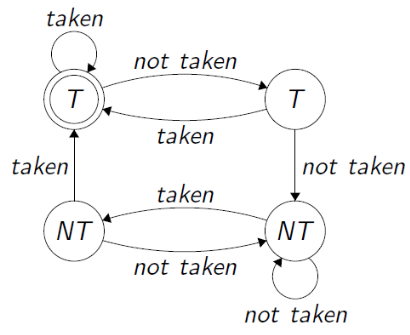
\includegraphics[scale=0.7]{immagini/2bit_pred}\\\\
si possono usare due bit per decidere come spostarsi in base alla predizione. Come si comporta con dei cicli annidati? 
\begin{lstlisting}
	mov $0, %ecx
.outerLoop:
	cmp $10, %ecx
	je .done
	mov $0, %ebx
.innerLoop:
	; actual code
	inc %ebx
	cmp $10, %ebx
	jnz .innerLoop
	
	inc %ecx
	jmp .outerLoop
.done:
\end{lstlisting}
L'unità per la branch prediction continuerà a dire branch taken finché non si arriva a 10, alla fine c'è una decisione sbagliata e si torna al loop esterno. Si cambia continuamente idea per via dell'interazione fra loop interno e loop esterno, per via di questo il 2-bit saturating counter non funziona bene perché sbaglia sempre la prima predizione e l'ultima.\\ La branch prediction è importante, perché da un'analisi risulta che nel codice il 20\% delle istruzioni sono branch condizionali, inoltre ci sono pipeline più complesse e super-scalari, quindi la possibilità di trovare delle istruzioni condizionali è più alta ed inoltre c'è la programmazione ad oggetti, dove per capire se una classe è figlia di un altra bisogna navigare l'albero per capire la classe padre e quindi prendere decisioni.\\ Per migliorare la branch prediction:
\begin{itemize}
\item migliorare la predizione
\item determinare il target prima
\item ridurre la penalità per predizioni errate
\end{itemize}
\subsection{Correlated prediction}
L'idea è che alcuni outcome dei branch sono correlati fra loro, quindi serve poter corralre due branch condizionali in assembly. In un correlated predictor si usa una storia degli m branch passati e si può usare la storia per correlare i branch. Si usa la path history table:
\begin{itemize}
\item si mette la storia globale in un registro globale della storia
\item si usa il valore per accedere ad una pht di 2-bit saturing 
\end{itemize}
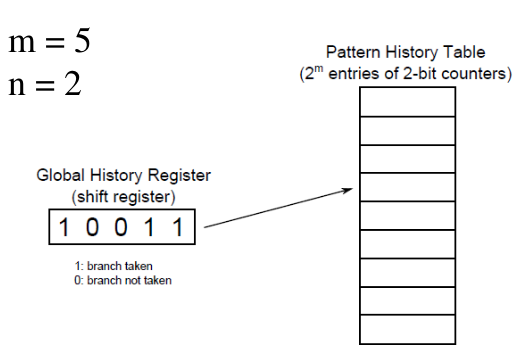
\includegraphics[scale=0.5]{immagini/corr_pred}
\subsection{Tournament predictor}
Si usano due tipi di predittori:
\begin{itemize}
\item correlated predictor, basato sugli ultimi m branches, acceduto dalla storia locale
\item local predictor, che viene selezionato usando l'indirizzo del branch
\end{itemize}
Si usa poi un indicatore di quale è stato il miglior predittore per lo specifico branch in esecuzione, che è un contatore a 2 bit, incrementato per uno dei predittori e decrementato per l'altro. Di seguito, uno schema dell'architettura del tournament predictor DEC Alpha 21264\\\\
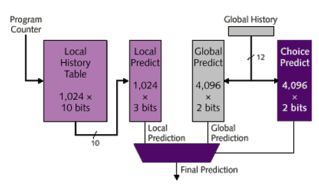
\includegraphics[scale=1]{immagini/tourn_pred}
\subsubsection{Branch target buffer}
È relazionato ai jump indiretti, che sono difficili da predirre. esempio: la ret è l'istruzione di ritorno da una sub routine. Il problema è capire dove si ritorna: qual è l'istruzione che si mette in pipeline, dovrebbe essere la prossima del chiamante ma è ancora più complicato. Si può fare il jump nell'indirizzo contenuto in un registro, l'output dipende da cosa è scritto nel registro che si vuole usare per il salto.\\ Il BTB è una picccola cache che viene acceduta col program counter 
%immagine dell'architettura
troviamo il prefetched target ed il prediction bit, che dice se conviene prendere il trarget oppure mettere uno stallo. È una cache, quindi ci può essere miss o hit, si può imparare se il prefetched target dovrebbe essere quello e più tardi si saprà se quel target è corretto o meno.
\subsubsection{Return address stack}
L'istruzione di ret legge l'indrizzo dallo stack, quindi se possiamo leggerlo subito possiamo sapere il target del ritorno.\\ Possiamo mettere uno stack nella CPU che manitene gli indirizzi di ritorno, ogni volta che c'è una chiamata, si salva in questo stack l'indirizzo di ritorno. In questo modo, ogni volta che si torna si conosce l'indirizzo di ritorno e questo è utilissimo perché l'85\% delle istruzioni è di ritorno.
\subsubsection{Fetch Both Target}
Tecnica che costa molto perché riempi la pipeline con tutte le istruzioni, ma la metà verranno scaratate e non aiuta in casi di fetch multipli come lo \textsf{switch}, non viene usato nell'hardware off the shelf.
%slides
\subsection{Simultaneus multi-threading}
C'è una CPU fisica ma è esposta al software come una coppia di CPU virtuali. L'idea è che mentre runni istruzioni nella pipeline usi un sotto-insieme delle risorse hardware, in questo caso nel simultaneous MT si puà tenere traccia di che hw stanno usando le istruzioni, quindi si duplica lo stato dell'architettura, quindi ad esempio il PC in modo che il processore usi un algoritmo di scheduling in modo da dare il controllo ai differenti thread che girano. Quindi è richiesto meno hw per far girare più processi ma servono dei controlli per evitare l'interferenza.
\subsubsection{Caso Intel: Hyperthreading}
Gli obiettivi sono molteplici:
\begin{itemize}
\item minimizzare la die area
\item evitare che uno dei due processori logici produca stalli per l'altro
\item "spegnere" l'hyperthreading se non necessario
\end{itemize}
Oggi, anche l'archiettura Inter mostra delle istruzioni assembly al programmatore diverse da quelle efeftivamente usate internamente, ci sono due parti:
\begin{itemize}
\item un front-end
\item un engine di esecuzione out-of-order: se puoi eseguire una micro operazione va eseguita immediatamente.
\end{itemize}
\paragraph{Xeon frontend:}il ruolo è quello di tradurre istruzioni CISC in istruzioni RISC usando una microcode ROM. C'è una cache di micro operazioni che mantiene le traduzione già fatte.\\ Nella trace cache, sappiamo se una micro operazione è associata ad uno o all'altro execution program, grazie ai due program counter differenti. Ci sono quindi due code diverse di micro operation. Nel caso di hit: %slides
\\ Nel caso di miss nella TC, serve fare la traduzione: bisogna accedere all'instruction TLB che permette di tradurre la corrispondenza fra indirizzi logici e fisici. Ovviamente, ci sono due TLB associati alla cache L2, quindi si può pagare anche un miss dovuto alla L2. Quindi, si mette la CISC instruction in coda, c'è poi il decoder ROM che mette le istruzioni in una coda usata per fillare la TC e quindi ora si può mettere la micro operation nella $\mu$op queue.
%slides
\paragraph{Xeon Out-of-order pipeline:}
%immagine
vogliamo eseguire le micro operazioni in ogni ordine quando è possibile farlo. Nel primo stadio, vogliamo schedulare i registri fisici della CPU: una $\mu$op cerca di accedere il registro icx, non è uno solo ma sono molteplici, i multi-registri e quindi icx viene mappato su uno di questi. Servono quindi un register rename ed un Allocate per tenere traccia di tutto.\\ Ora ci sono code multiple, per discriminare la semantica della $\mu$op in base al fatto che si acceda alla memoria etc...\\ Lo stadio di execute ha diverse ALU, quindi l'Allocation unit dice anche quale componente usare per eseguire l'istruzione. Lo scheduler prende l'istruzione dalla coda nel momento esatto in cui il componente è disponibile. L'ordine è qualsiasi, le $\mu$op appartengono a diversi program flow, quindi data una CISC operation, le macro istruzioni saranno invertite nell'ordine. \\ Alla fine, non vogliamo che le istruzioni siano materializzate all'esterno in ordine casuale, quindi c'è un reorder buffer per riordinare le istruzioni CISC nell'ordine in cui sono entrare e far credere all'utente siano state processate così.\\ Non abbiamo quindi una idea di come siano state eseguite le istruzioni internamente, quindi ci può essere uno stato di inconsitenza per un tempo illimitato ma non è un problema perché questo non viene esposto a livello ISA. Il problema è che stiamo interagendo con la memoria e questo è sfruttabile, possiamo ad esempio far si che la CPU carichi delle istruzioni che non doverebbe e quindi dei dati in cache che non dovrebbe: l'istruzione non verrà committata, ma la traccia sarà comunque esposta e sfruttabile.
\subsection{Multicores (2000s)}
I vendor cominiano ad usare i molteplici tansistor per creare delle CPU multicore, il primo CPU è l'IBM power4, 2 core con una architettura interessante: una cache privata per ciascun core, interconnessione di un certo tipo fra i core e una cache di L2 ed L3, dove la L3 fa anche da memory controller. I core interagiscono con la L1 e così a salire, quindi per caricare dati dalla memoria. Ma sei i cores hanno una cache privata, come fanno ad essere sincronizzati con i dati contenuti in L1 e quindi visibili al core 2? Serve un protocollo apposito per garantire la consistenza dei dati.
\subsubsection{Cache coherence}
Comportamento della cache da un punto di vista di utilizzo. La CC definisce la coerenza della cache con dei protocolli: quando scrivo codice, non mi rendo conto di interagire con la cache, ma i processori vi interagiscono di conitnuo. Abbiamo ad esempio 2 cores, con due cache private ed una serie di operazioni:
%carica la tabellina
al tempo 0, la cache del core 1 c'è la copia di A, a t=1 C2 carica A in un altro registro. Poi C1 fa una una operazione su A, quindi il valore di A nella cache di C2 quale sarà? Non c'è una sola risposta, dipenderà dal protocollo di consistenza
\paragraph{Strong CC protol:}il protocollo più semplice, tutte le cache dei vedono gli stessi dati, come se non ci fosse una separazione fra le cache in un qualunque istante di tempo. Quindi, serve avere un agreement fra i cores su chi fa l'operazione sul dato, quindi c'è un impatto sulla concorrenza e le perfomance.\\ Per assicurare tale consitenza serve:
\begin{itemize}
\item single write/multiple readers: ad ogni istante di tempo, per ogni locazione di memoria un solo core può leggere e scrivere
\item (slides)
\end{itemize}
Bisogna continuamente sincronizzare le cache quando un core fa un update in memoria, quindi non è molto performante
\paragraph{Coerenza debole:} c'è meno limitazione sulle cache, in quanto devono sincronizzarsi meno, quindi viene persa una delle invarianti dette sopra. Quindi due cores possono scrivere su una stessa area di memoria, quindi può accadere che il programmatore osservi dei comportamenti inattesi e quindi per implementare correttamente l'algoritmo occorre implementare delle primitive software per avere lo stesso outcome che si avrebbe se tutto accadesse sequenzialmente.\\ C'è una time window di un certo numero di epoche temporali in cui i dati non vengono propagati e questo può mostrare la complessità dell'hardware al programmatore\\\\ È anche possibile non avere coerenza, che è il modo per avere le cache più veloci. Non ci sono ovviamente garanzie, quindi le cache vanno sincronizzate esplicitamente lato software, ad esempio con delle API C/Assembly.
\subsubsection{CC protocol}
Un protocollo di consitenza per la cache è un algoritmo distribuito basato su primitive di tipo message-passing. Ci sono due principali tipi di richieste in memoria da servire:
\begin{itemize}
\item Load(A)
\item Store(A)
\end{itemize}
e coinvolge 2 tipi di attori principali, ovvero i cache controllers ed i memory controllers. Il ruolo è quello di rinforzare una certa nozione di coerenza.\\ Qualunque cosa nei protocolli CC è basato sulle coherency transaction, ciascuna di queste genere dei messaggi. Ci sono due tipi principali di transazioni:
\begin{itemize}
\item Get: carica un blocco di cache (dato) in una linea di cache
\item Put: evince un blocco dalla linea di cache, la linea diventa disponbile per altri dati
\end{itemize}
%immagine dell'organizzazione
Ogni linea di cache è associata con un bit che dice se la linea è valida o memo, in questo caso abbiamo una macchina a stati finiti che definisce lo stato del blocco in cache. La macchina è leggermente più complessa di una classi FSM, perché per transitare dai vari stati ci possono essere dei delay dovuti al fatto che il protocollo è distribuito. Ci sono quindi
\begin{itemize}
\item eventi remoti: viene ricevuto un messaggio di coerenza
\item eventi locali, ricevuti dalla parent cache
\end{itemize}
(altro sulle slides)\\ Ci sono una serie di protocolli per gestire la coerenza, definiamo
\begin{itemize}
\item invalidate protocols: protocolli, quando viene scritto un blocco invalida tutte le altre copie.
\item update protocols: ogni update viene mandato a tutti i core.
\end{itemize}
Quindi, nell'esempio iniziale il valore di A dipende dal protocollo implementato. Ci sono poi due famiglie di CC protcolos diversi
\begin{itemize}
\item snooping protocols: tutti i controller osservano tutto il traffico, quindi il broadcast è totalmente ordinato. È molto veloce, perché tutti i controller possono fare decisioni da soli perché osservano tutti i messaggi ma non è scalabile se il numero di core aumenta. Questo perché serve una arbitro del bus, e questo degrada le performance
%immagine snooping
\item directory based: c'è una directory, ogni request è unicast alla directory. Questa tiene traccia di chi è il controller destinatario e gli manda il messaggio, il che rende tutto più scalabile e permette di aumentare il numero di cores.
%immagine directory based
\end{itemize}
\subsubsection{VI protocol}
Il protocollo di consitenza più semplice, un solo cache controller può leggere e/o scrivere il blocco in ogni timestamp.\\ La transaction Get è usata per richiedere un blocco in read-mode per poter diventarne l'owner e potervi scrivere e leggere. La Put è usata per togliere il blocco dalla cache e riscriverlo al LLC controller. Ci sono una serie di eventi:
%copia slides
Il protocollo VI sta per Valid/Invalid, ma oltre a questi due stati ce n'è anche uno intermedio per cui si aspetta una copia del dato up-to-date
%immagine del FSM
Se confrontata con la FSM del LLC, vediamo che c'è differenza: ad un certo punto, il core associato al cache controller fa una operazione di load, quindi ottiene l'indirizzo e va nella cache e scopre che lo stato della cache è I. Quindi, serve una Own-Get dal LCC, manda un messaggio che viene ricevuto da tutti i cache controller nel sistema con un ordinamento totale. Una volta che il messaggio viene mandato, il controller trainsita nello stato IV, la copia verrà inviata dal possessore attuale del dato, dopo averlo ricevuto transita in V. \\ Dopo, un altro core vorrà diventare l'owner e quindi questo controller transiterà nello stato I e trasferirà il contenuto del blocco.\\ Immaginiamo di essere in una situazione in cui c'è un conflitto, ovvero si vuole scrivere un blocco nella linea di cache che è piena. Si manda una Any Put al LLC controller, l'LLC transita nello stato I e se poi qualcuno richiede il dato transita nello stato V.\\ Il protocollo ha una nozione implicita di diryness: se una linea di cache è in stato V, il controller L1 può o leggere e scrivere o solo leggere. Ha anche un concetto implicito di esclusività, in quanto se lo stato è V, nessun altro può accedere al blocco, quindi nessuno ha una copia valida; inoltre, c'è nozione del possesso del blocco: l'owner sarà quello che manda la copia aggiornata a tutti.\\ La cosa positiva del portocollo è che richiede pochi bits per rappresentare le FSM, ma ha diverse inefficienze; ciò che vogliamo catturare del blocco di cache sono aspetti di
\begin{itemize}
\item validità
\item dirtyness
\item exclusivity
\item ownership
\end{itemize}
vogliamo solo queste proprietà per avere un protocollo efficiente ma che consumi più bits per l'implementazione
\subsubsection{MOEST stable states}
Ogni lettera fa riferimento ad uno stato particolare, ognuno cattura una delle proprità dette sopra. Di nuovo, è una FSM per ogni blocco
\begin{itemize}
\item Modified: il blocco è valido, esclusivo, posseduto e potenzialmente dirty.Può essere scritto o letto
\item Owned: blocco valido, posseduto 
\item Shared: valido, non esclusivo, non posseduto, non sporco. Ci sono più copie read only del blocco.
\end{itemize}
(slides)\\ Quali sono le transazioni per poter implementare il protocollo:
\begin{itemize}
\item GetS: Get del blocco in Shared state
\item GetM: Get in modo Modified
\item Upgr: ho un blocco, so che il blocco ha la copia più aggiornata perché ho osservato le transazioni, quindi non voglio la copia del dato ma voglio la possibilità di scrivervi
\item Put (slides)
\end{itemize}
Questa è la macchina a stati che si ha tipicamente: 
%immagine della macchina
\subsubsection{MEST protocol}
Il controller della cache di livello inferiore (LLC) è simile 
%immagine
M/E è uno stato congiunto di Modified/Exclusive. Se in M/E e si osserva una Any-Get, si va in Shared, se qualcuno richiede il blocco, si va in I.
\subsection{Memory Control}
Nelle cache write through, si propaga direttamente l'update.\\ In modern architectures, the cache are no longer write through, due to the complexity can explode.\\ The caches in modern architectures can be either inclusives or exclusives at different levels, this can be exploited by attacks that specifically targets a L* cache.\\ CC dicatates how the different cache controllers interacts among them. There is the concept of memory consistence: il MC model definsce il comportamentio di una memoria condivisa, indipendentemente da come è implementata. Vediamo ancora un esempio:
%tabella esempio
in macchine Multi Core c'è il riordino degli accessi in memoria: il core committa le operazioni sulla memoria in un certo ordine ma gli altri cores possono osservarle in ordine diverso, quindi non c'è un ordinamento totale. Il sotto-sistema può quindi riordinare le operazioni: 
%tabella di esempio
ci sono 4 combinazioni di possibili riordini, quindi se scriviamo codice concorrente, dobbiamo considerare il fatto che ci siano riordini delle operazioni.\\ Questo ha a che fare con due ordinamenti diversi:
\begin{itemize}
\item ordiamento di programma, è per core ed è totale. Cattura l'ordine in cui ogni core 
\item ordinamento di memoria (slides)
\end{itemize}
Possiamo avere diverse consistenze:
\begin{itemize}
\item sequenziale: ci sono determiante operazioni che verranno osservate identicamente tra ordine di programma ed ordine di memoria.\\ Nell'esempio di prima, solo due ordini sono consitenti sequenzialmente
\item consitenza debole: modello implementato dalle architetture moderne. Quella di Intel è Total Order Store. C'è un piccolo buffer che agisce come coda in cui vengono salvate le diverse operazioni di store e che verranno poi processate. Le architetture Intel sono fra quelle in cui c'è il minimo numero di riordini tra le operazioni
\end{itemize}
\subsubsection{Memory fence}
Se ho una qualunque operazioni di memoria, la fence forza l'ordine di una load/store, quindi possiamo creare dei punti in cui siamo sicuri che tutte le istruzioni prima della fence sarà ordinata e stessa cosa se accade prima, ma non si possono riordinare le fence. Sono quindi operazioni speciali che permettono di mettere dei punti di riordino per poter ad esempio avere consistenza sequenziale in Intel.
\paragraph{Fence su architetture x86:} ci sono 3 tipi di fence diverse su x86:
\begin{itemize}
\item MFENCE: barriera full memory, ogni operazione prima e dopo non sarà riordinata
\item SFENCE: barriera store/store
\item LFENCE: barriere load/load e Load/Store
\end{itemize}
\section{In memory transaction}
Le transazioni in memory permettono di realizzare la sincronizzazione in memoria più semplice. Può essere esplicita, quindi per accedere ad un sezione critica si prende un lock, si accede e poi si esce.\\ Ci possono essere problemi sui locks come deadlock, i deadlocks non sono componibili e quindi possono esserci delle inconsistenze nei risultati di operazioni che usano i lock.\\ L'hardware transactional Memory prevede di usare delle istruzioni di Assembly specifiche per dire che su vuole accedere a dei dati in maniera esclusiva, così che il processore metta un lock privato sui dati e una volta finito, se il commit va a buon fine i dati vengano pubblicati all'esterno\\ Per poter implementare le hw transaction Intel ha modificato il protocollo di CC: i tentativi vengono fatti solo al primo livello della cache e si marcano i blocchi di cache con lock, per poi committare se va tutto bene. Ci sono 4 nuove istruzioni Assembly (slides), esempio in C:
% codice del C ed Assembly
Una transazione può andare in abort per vari motivi (slides)\\ Da un punto di vista di performance il problema è per cosa di fa abort a livello hardware, ma la cosa interessante è che la transazione può essere mandata in abort da qualunque altro CPU core.
Se mettiamo di mettere del codice per fare delle transazioni, rischiamo che dopo se mettiamo del codice su quello scritto per fare i lock possiamo avere una esecuzione per cui in concorrenza le cose non tornato (vedi l'esempio dei depositi/ritiri sulle slides), perché i lock non si compongono.\\ Si possono usare le transazioni, concetto preso dal DBMS: quindi, vogliamo eseguire tutte le operazioni fra l'inizio e la fine di una transazione come all or nothing, È possibile farlo sia usando un DBMS, sia tramite l'uso di facilities offerte dall'hardware.\\ La facility hardware è quella delle \textbf{Hardware Transaction Memory}: l'idea dietro è che se nulla va storto, si hanno delle performance migliori. Usati molto negli engine per videogiochi, quasi tutti i processori off the shelf offrono transactional memory, Intel li ha disabilitati quasi del tutto per via di una implementazione buggy.\\ Il paradigma HDM lavora in questo modo:
\begin{itemize}
\item introdurre operazioni Assembly per capire quando inizia e finisce la transazione
\item utilizzo delle cache, i controller sono già in grado di capire se operazioni concorrenti stanno accedendo allo stesso dato e quindi se scoprono un conflitto sui dati, droppano il flusso di esecuzione ed anche i side effects sui dati. Ci sarà poi un retry path
\end{itemize}
Il tipico hardware off the shelf è mostrato di seguito, usato per fare il reverse engineering di come è fatto l'HTM
%immagine dalle slides
la L1 e la L3 possono essere usate per implementare le transazioni, in quanto possono essere usate per rappresentare le transazioni. Ci sono due gruppi di dati, read set e write set. L'implementazione delle HTM introduce un bit aggiuntivo per ogni cache line, che dice se un blocco è stato caricato o letto durante una transazione.\\ Il protocollo di CC sa quali linee sono marcate come transaction access, se se ci sono concorrenze e può agire per rendere lo stato coerente. (slides)
\subsection{Funzionamento}
Le istruzioni assembly usare per supportare HTM sono
\begin{itemize}
\item \textsf{xbegin}
\item \textsf{xend}
\item \textsf{xabort}
\item \textsf{xtest}
\end{itemize}
(vedi slides per dettagli). La cosa buona di questa implemetazione è che sulla base di queste 4 operazioni è possibile scrivere delle transazioni annidate, il che rende la scrittura del codice molto più semplice; il CC controller tiene un contatore delle nested transaction fatte, quando il valore va a 0 pulirà i bit dalla cache.\\ Tutti i compilatori moderni possono generare queste 4 transazioni, a partire da linguaggi di alto livello come C e C++, generando delle Undefined Instruction se HTM è implementato in hardware.\\ Per usare le operazioni, si può scrivere del codice C:
%codice dalle slides.
È possibile capire anche se c'è un abort in corso, quindi è utile se abbiamo una transazione grossa capire se c'è un abort perché magari il processore non è in grado di portarla a commit.\\ Il write set è vicino alla CPU, sta nella L1, mentre il read set è sia in L2 che in L3. Quindi, il cache controller setta il T flag sia in L1 che in L3 quando si legge, mentre solo in L1 quando si scrive. Supponiamo di avere l'esempio del bank account: se ci sono due diversi cache controllers che stanno gestendo le transazioni, non possono conoscere lo stato l'uno dell'altro ma possono verificare che ci sia un accesso concorrente e quindi se ogni altra CPU legge una location di un write set, la transazione andrà in abort: c'è un pezzo dati che è marcato con T, non è ancora committata ed il controller deve mandare il dato più fresco e se c'è una read non può mandare il dato fresco e quindi la transazione deve abortire.\\ Vale lo stesso per le altre CPU: se qualcuno scrive in un read o write set, la transazione va in abort, l'algoritmo è quindi locale al controller, può dare delle performance peggiori per via che si mandano in abort anche cose che non dovrebbero. \\Inoltre ci sono anche limitazioni hw, cosa accade se abbiamo un contex switch: non possiamo lasciare dei dati incommittati nella cache, quindi la transazione deve abortire e lo stesso vale per la ricezione di un interrupt, perché non si sa per quanto tempo si starà in questo stato e non si possono lasciare i dati inconsistenti; lo stesso vale per page faults.\\ Quindi è necessario avere della logica di codice per gestire gli abort\\ I codici di errore possono essere vari
\textbf{esempio:}\\ abbiamo una transazione, vediamo l'effetto sulla cache
%codice dell'esempio
Abbiamo solo due locazioni di memoria coinvolte nella transazione, vediamo cosa accade in una possibile run concorrente:
\begin{itemize}
\item $CPU_0$ legge $a_0$ dalla cache e setta il T bit
\item $CPU_0$ scrive su $a_0$, portando quindi lo stato a modified, quindi $a_0$ è nel write set
\item $CPU_1$ legge $a_1$ nella cache (in maniera esclusiva) e setta il T bit
\end{itemize}
Lo stato della cache è il seguente:
%slides
quindi è possibile committare semplicemente pulendo lo stato dei bit.\\ Se $CPU_1$ entra in gioco e legge $a_0$, la $CPU_0$ deve per forza fare abort: pulisce i T bit e rende le linee di cache invalide che erano Modified. Ora, $CPU_1$ deve per forza leggere i dati dalla memoria, perché in cache sono invalide, questo avviene proprio quando $CPU_0$ stava per fare il commit.
\section{Recap sulla gestione della memoria virtuale}
La memoria virtuale serve per far si che le applicazioni non accedano alla memoria fisica direttamente, bensì tramite degli indirizzi virtuali. L'idea è do astrarre cosa una applicazione vede e cosa il processore dovrebbe fare, per molteplici motivi
\begin{itemize}
\item rendere la scrittura del codice più facile;
\item ingannare l'applicazione, facendole credere di avere più memoria in quanto si può fare lo swapping sulla memoria;
\item isolamento per processo: se qualcuno nel sistema può trasformare un indirizzo virtuale in uno fisico ed il componente è abbastanza sicuro, ci sono delle delimitazioni che impediscono ai processi di vedere i dati di altri processi, a meno di usare memoria condivisa
\end{itemize}
Il supporto alla memoria virtuale usa sia hardware che firmware, che OS (slides).\\ Usiamo la terminologia di virtual page e di segmento di memoria: una pagina virtuale viene mappata su un un frame fisico.
%immagini
è possibile che un certo range degli indirizzi virtuali condividano dei frame fisici in memoria. IL firmware deve fare diverse operazioni per poter usare le pagine virtuali, quindi viene introdotto una cache addizionale per facilitare la traduzione tra virtual e phisical address: TLB, che se ha la traduzione in memoria da l'indirizzo fisico corrispondente all'indirizzo virtuale.\\ I passi della traduzione sono riassunti di seguito:
%immagine slide
si può avere un indirizzo virtuale valido, che però non è presente nella memoria fisica per via dello swapping, quindi si ha un miss nel TLB o nella page table.
\subsection{Traduzione in x86}
Le CPU Intel sono bloated, quindi cercano di fare di tutto per dare retro-compatibilità, quindi ogni volta che c'è una nuova facility viene disabilitata per default, quando parte un nuovo chip Intel è come se fosse un 8086, ci pensa il SO ad abilitare tutto ciò che serve:
\begin{itemize}
\item segmentazione di memoria
\item segmentazione di memoria in protected mode
\item paginazione
\end{itemize}
L'indirizzamento basata sulla segmentazione è fatta in base a questo schema:
%immagine dalle slides
Come funziona l'unità di segmentazione: 4 registri a 16 bit (allo startup girano così) per i segmenti
\begin{itemize}
\item CS: code segment, dove trovare il codice in memoria
\item DS: data segment, dove trovare i dati in memoria
\item SS: stack segment
\item ES: extra segment
\end{itemize}
Intel i386 ha aggiunto due nuovi registri, FS e GS senza uso predefinito.\\ Basandosi sulla segmentazione, si possono definire dei segmenti di memoria in cui ogni segmento è un numero che indica l'inizio del segmento, quindi è possibile avere overlapping. Un esempio è mostrato in seguito:
%immagine delle istruzioni Assembly dalle slides
\subsubsection{Registri x86\_64}
%immagine dei registri
fra i tanti registi, i due di interesse sono (slides). Abbiamo bisogno di strutture dati, che è un virtual-to-phisical tree che mantiene le tabelle di traduzione e la cui root è indicizzata da CR3.
\subsubsection{Segmentazione protected mode}
%immagine
tra le informazioni che otteniamo, dovremmo avere la base dell'indirizzo ma in realtà si ha un indice che serve per accedere ad un tabella in memoria centrale. La tabella ha dei segment descriptor che mantengono i base address per i segmenti,può essere ovunque in memoria per cui si può avere l'indirizzo nel registro GDTR. Supponiamo di avere una jmp che ha un target: l'indirizzo diventa un offset, nel CS register si trova un indice nella global descriptor table. A quel punto si usa l'index come offset nella tabella e trova il segment descriptror, quindi si prende la base e si somma all'offset per ottenere un indirizzo logico.\\ La base è sempre 0, per via della retro-compatibilità, ma il processo va comunque fatto per rendere possibile la paginazione (lo fa il SO). Quando rendiamo possibile la paginazione, l'indirizzo è lineare e viene passato all'unità di paginazione (firmware) che lo trasforma in un indirizzo fisico e lo passa alla CPU
\subsubsection{Unità di paginazione}
L'idea è che l'indirizzo lineare viene diviso in 3 pezzi (32 bit):
\begin{itemize}
\item directory: indice alla tabella puntata da CR3
\item Table: indice nella page table
\item offset, che viene usato per trovare l'indirizzo fisico del frame
\end{itemize}
%immagine
ogni tabella ha nel record un puntatore al componente successivo, sono tutte mantenute in memoria e la gestione è fatta dal SO. C'è un albero di tabelle per ogni processo. Quando si fa context switch, il valore del CR3 non viene cambiato e quindi è possibile anche trovare indirizzi del kernel.
\subsection{Traduzione Virtual-to-phisical i386}
L'istruzione assembly ha un indirizzo logico, che verrà usato come offset per la tabella dall'unità di segmentazione per ottenere un indirizzo logico, che verrà usato dalla page table per navigare una pagina ed ottenere un indirizzo fisico da passare alla CPU. Ogni volta che si accede ad un singolo byte di memoria si triggera tutto il processo
%immagine
quindi per questo è stato introdotto il caching, per cercare di ridurre la latenza. Per usare l'indirizzo fisico, il cache controller deve aspettare che tutta la traduzione avvenga, se si usa solo l'indirizzo logico c'è un problema se le tabelle cambiano.\\ È possibile usare entrambe le cose: appena l'applicazione genera un indirizzo lineare, questo viene preso dal firmware del cache controller L1, e se il dato è in memoria c'è un hit. In parallelo c'è il controllo nel TLB per vedere se è possibile tradurre in indirizzo fisico. Se c'è un miss nel TLB parte la traduzione per ottenere l'indirizzo. Quindi diversi livelli di cache sono indicizzati con diversi indirizzi, per cercare di velocizzare il processo di traduzione si fanno diverse cose in parallelo.
%immagine riassuntiva
\section{Primitive di lettura}
Vogliamo trovare un modo per bypassare l'isolamento dei processi, la tecnica da usare sarà il timing: vogliamo mettere su delle primitive di lettura, l'idea fondamentale dietro la sicurezza è che non vogliamo lasciare delle informazioni, a volte anche il tempo impiegato per fare un'operazione dice qualcosa. 
\subsection{Algorithm Timing}
Prendiamo il seguente esempio:
\begin{lstlisting}
int strcmp(char *t, char *s){
	for( ; *t == *s ; s++, t++){
		if(*t == '\0')
			return 0;	
	}
	return *t - *s;
}
\end{lstlisting}
passando le due stringhe "ABCD" ed "ABxDE" possiamo inferire qualcosa dai dati in base al tempo impiegato per fare il confronto.\\ Useremo degli approcci simili sulla cache: ogni volta che leggiamo i dati dalla CPU, questi vengono letti dalla cache e quindi ogni volta che si fa una load, a seconda della della condizione, ci saranno differenti risultati
\begin{itemize}
\item supponiamo di avere la cache in modified, siamo i proprietari e possiamo leggere
\item se il blocco è invalid, occorre fare altre azioni
\end{itemize}
dipende tutto dallo stato in cui è la FSM della cache. L'idea è che possiamo fare delle operazioni sulla cache privata in modo da portare la FSM in degli stati che conosciamo, quindi per fare un side channel
\begin{itemize}
\item portiamo la cache in uno stato noto
\item facciamo si che qualcuno faccia delle operazioni sulla cache per cambiarne lo stato
\item vediamo, tramite timing, come è cambiato lo stato
\end{itemize}
con l'hyperthreading è ancora più critico, perché ci sono più thread che girano sullo stesso core e quindi condividono la stessa cache L1 e quindi potremmo leggere i dati di qualcun altro e quindi violare la privatezza della L1 per via del simultaneous MT; ((NB: se non ci fosse, la L1 rimarrebbe privata. Inoltre, la L1 di usa indirizzi virtuali per indicizzare i blocchi dati, quindi è anche più semplice accedere ai dati.))
\subsection{Code path}
Ci sono degli algoritmi su cui non si può fare timing, perché l'algoritmo ci metterà sempre lo stesso tempo. Ad esempio abbiamo il Montgomery Ladder, usato per fare operazioni sulle curve ellittiche e blocco chiave della crittografia. Abbiamo delle nonce, che devono essere univoche altrimenti si potrebbe invertire la curva (ricavare la chiave privata), lo pseudocode è il seguente:
%codice dell'algoritmo
abbiamo k bit, ma il numero di operazioni è sempre lo stesso. Accediamo allo scalar, 1 bit alla volta, ed a seconda del valore accediamo ad uno dei rami dell'if-else e quindi ci chiediamo se possiamo determinare in quale dei due branch siamo, sfruttando la L1 per ricavare la nonce. Una volta che il codice è caricato, viene messo in cache ed alcune operazioni sono grandi e quindi finiscono su più linee di cache, quindi se riusciamo a portare lo stato della gerarchia della cache in modo da capire in quali linee di cache è stato eseguita l'operazione, possiamo sapere se è stato preso l'if o l'else.\\ Quindi, anche se l'algoritmo è time independent, possiamo osservare quali linee di cache sono state usate per accedere ai dati
\subsection{Side channel attacks}
Un side channel è una zona di memoria che permette di leggere un altro contenuto di memoria o accedere a dei pattern di dati. Ci sono diverse tipologie di side channels
\begin{itemize}
\item Prime + Probe
\item Flush and Reload
\item Flush + Flush
\item Evict + Time
(slides)
\end{itemize}
l'idea è sempre che la prima parte viene usata per portare la cache in un certo stato, con la seconda si cerca di capire dopo che la vittima ha fatto qualcosa, qual è il side effect sullo stato della cache. Non c'è nulla che il SO può fare per garantire l'isolamento dei processi, perché lo stato dell'hardware è condiviso. Un attacco passa per diversi stati, le differenti macchine cambiano per diversi aspetti quindi abbiamo
\begin{enumerate}
\item pre-attack: il pre-target attack serve per acquisire il target, quindi ad esempio la linea di cache o il cache set (nel caso di cache n-associative ) stabilire eventuali timing threshold. Dobbiamo considerare tanti elementi, come ad esempio il carico di lavoro della macchina, se è alto potremmo essere deschedulati e perdere ad esempio la CPU su cui stavamo lavorando venendo rischedulati su un'altra
\item active attack:
\begin{itemize}
\item[a)] Inizializzazione: portare il canale in uno stato noto
\item[b)] Attendere che la vittima faccia un accesso in memoria
\item[c)] Analizzare l'accesso, osservando i side effects lasciati dalla vittima
\item[d)] Ripetere l'accesso fino al leak dei dati
\end{itemize}
\end{enumerate}
Ci sono diversi aspetti da considerare
\begin{itemize}
\item Le cache sono cachate sia virtualmente che fisicamente
\item le cache sono condivise in maniera differente in base al livello
\item vanno considerati anche gli interleave di esecuzione fra i diversi processi
\end{itemize}
mettere su un vero side channel attack è molto più complesso di cosa si legge nei paper
\subsubsection{Evict + Time}
Il target è la cancellazione di una linea, quindi inizialmente la vittima gira e fa degli accessi in memoria, quindi carica i suoi dati in memoria. A questo punto, stabiliamo una baseline execution, ovvero sappiamo che la vittima girerà di nuovo e quanto ci metterà quando ha i dati in cache. L'attacker quindi cancella una linea di interesse dalla cache per scoprire se la vittima la usa: in algoritmi crittografici, si ci basa su tabelle di dati condivise che vengono usati in base alla chiave. Quindi se sappiamo quale parte della tabella viene usata, possiamo fare una ricostruzione di discovery code path, quindi capire quale parte dell'algoritmo viene usato mentre gira. Questo stato effettivamente usato per rompere AES, possiamo scoprire quali linee di cache sono state usate per capire ad esempio la chiave di cifratura, usando il tempo: vediamo quanto ci vuole per fare degli accessi per capire se la vittima sta usando una cache line cancellata o no.\\ La parte critica è poter far girare la vittima quando si vuole, ad esempio è stato usato per rompere AES perché è una libreria condivisa e quindi è possibile per l'attaccante far girare la vittima.\\ Non usare solo l'istruzione Assembly \textsf{rdtsc} per contare il tempo che passa, i chip del processore vengono spenti/accesi in base alla temperatura del processore (perché si tocca il power wall) così come anche viene \textbf{decrementata la frequenza del processore}, quindi il numero di cicli effettivi contati è falsato. Usiamo l'istruzione \textsf{rdtscp} perché rispetta il program order, altrimenti bisognerebbe usare le fence (ricorda l'esempio di Quaglia). La cosa interessante è che l'attacco è veloce quanto la vittima è veloce nel computare.\\ Nota: nel codice, vengono usati buffer di caratteri di 4096 byte, perché? La gerarchia delle cache sono state introdotte nel calcolatore per sfruttare la località in modo da fare andare tutto più velocemente. Uno dei principi è la \textbf{località spaziale}, quindi possibilmente se viene caricata una linea di cache, anche se viene caricata una sola linea e quella successiva è associata ad uno stato invalid, la cache potrebbe pre-fetchare una linea di cache. Quindi, dobbiamo considerare il pre-fetching quando buildiamo un attacco, essendo sicuri che le linee pre-fetched vengano flushate. 4KB è una pagina ed è talmente grande che anche col pre-fetching siamo abbastanza sicuri che non ci siano effetti indesiderati dopo la flush della linea di cache.
\subsubsection{Flush + Reload}
Basato sull'abilità di usare memoria virtuale condivisa, quindi affinché funzioni il pre-requisito è che sia possibile condividere i dati virtualmente con un altro processo, quindi diverse applicazioni condividono pagine di memoria per risparmiare spazio (si usa la copy on write, appena si cambia un byte si duplica la pagina). Flushamo una linea di cache, possiamo farlo con un indirizzo virtuale, eseguiamo la vittima e poi proviamo a ricaricare le linee di cache flushate prima e misurare il tempo. Se flushamo la linea e viene ricaricata dopo un po', nessuno l'ha toccata, altrimenti vuol dire che una vittima ha toccato quella linea di cache e quindi una parte di dati. La vittima viene fatta girare una volta sola, se non c'è noise sulla gerarchia di cache basta girare una volta sola.\\ Nel codice, viene allineata la pagina di cache, la prima cosa che si fa è materializzare il vettore di probe in memoria: l'approccio di Linux è che il kernel non si fida dello sviluppatore, quindi se chiede molta memoria l'OS ne da di meno se si accorge che è fatto di zeri. Quindi, l'indirizzo di memoria virtuale è valido, ma non è mappato in memoria fisica del tutto, c'è una pagina in Linux che è piena di 0 (la zero page) che viene condivisa da tutte quelle strutture con tutti zeri. In questo modo si dice al kernel che si vogliono davvero le 256 pagine, semplicemente scrivendo un byte.\\ Ora, bisogna discriminare fra cache hit e miss e mettiamo delle lfence per essere sicuri che non ci sia della noise aggiuntiva per via della memory consistency.\\ NB: nell'attacco, creiamo una pagina per ogni singolo valore del byte che andiamo a leggere. Quindi nell'accesso in \textsf{make\_side\_effect} leggo una pagina della memoria prendendo uno qualsiasi dei valori del byte, quindi creo un pointer in una delle pagine del vettore che verrà portata in cache, che sarà associata al valore del byte. Se troviamo la pagina numero 0 in cache, vuol dire che il valore del byte è 0, se invece trovo la pagina 1, vuol dire che il byte letto è 1 e così via.\\ Quindi, mi baso su due cose
\begin{itemize}
\item uso la grandezza di una pagina per mitigare il cache pre-fetching
\item carico un valore in memoria senza far girare la vittima. Se ho l'indirizzo di memoria virtuale e posso leggere un valore in memoria, posso leggere un valore, portarlo in un vettore e poter vedere se quel byte viene acceduto
\end{itemize}
perché non leggere direttamente il valore del puntatore? L'indirizzo può essere valido, ma non è detto che siamo in grado di leggere perché non abbiamo privilegi di lettura in memoria.\\ Otteniamo un seg fault se la memoria non è valida, ma lo possiamo gestire con un handler e continuare con l'esecuzione e quindi possiamo bypassare i privilegi di accesso perché abbiamo portato dei dati in memoria. Questo è il fondamento di meltdown.
\subsubsection{Prime + Probe}
Si fa girare in cache L3, non serve per forza SMT, si può anche lavorare fra diverse VM. La tecnica prevede di fare un priming della cache, ovvero portarla in uno stato noto caricando dei dati che conosco in cache, mettendo uno o più linee di cache che riempano tutte le linee in quanto la cache è set-associativa.\\ Una volta fatta girare la vittima, questa deve invalidare delle linee di cache e carica i suoi valori, a questo punto possiamo rigirare e fare il probing del cache set caricato prima tramite una operazione di probing: se il tempo di accesso aumenta, sappiamo che la vittima ha toccato quelle linee di cache.\\ Un attacco di successo di Prime + Probe non è così semplice perché mettere su un cache set non è così semplice in una cache set-associativa
%immagine
Ci sono delle contromisure hardware, il mapping memory-to-cache cambia di continuo (slides)\\ L'unico modo per mettere su l'attacco è conoscere il mapping a run time:
\begin{itemize}
\item scegliere N indirizzi di memoria casuali. C'è la possibilità di un cache collision perché non conosciamo il mapping con la memoria
\item misuriamo il tempo che ci vuole per caricare la cache accedendo agli indirizzi di memoria
\item se becchiamo una self cache collision, rimuoviamo l'indirizzo dal set. Possiamo usare CPUID per capire l'architettura della cache
\end{itemize}
\subsubsection{Prime + Abort}
Permette di fare tutto ciò che è stato detto fin ora senza timing. Tramite le transactional memory, avremo delle hardware callback che ci dicono che c'è stato un accesso in memoria. L'idea è quella di fare una transazione, aspettare per un abort e nel momento in cui l'abort avviene sappiamo chi ha fatto l'accesso alla memoria (slides).\\ Possiamo anche mettere su degli attacchi alla cache L3: una linea di cache scritta durante una transazione viene tolta dalla L1, quindi l'accesso transazionale fa una write in memoria (slides)
\subsubsection{Flush + Flush}
La clfush non è idempotente rispetto al timing, quindi a seconda dell'input ci metterà tempo diverso. Facciamo una clflush e la CPU dice al cache controller di fare un flush ma a seconda dello stato della cache il tempo impiegato sarà diverso. È una versione del Flush + Reload che permette di capire se la cache line è stata invalidata da qualcuno. È molto stealthy come attacco, perché non si fa molto rumore ed inoltre è veloce. Quindi, anche la \textbf{bandwidth} dell'attacco è aumentata, perché il numero di dati che si riescono a scoprire è maggiore.
\section{Out of order pipeline}
Usando i side channel attacks visti, vediamo cosa possiamo fare introducendo la out of order exection pipeline: possiamo fare il leak dei dati, se facciamo girare le micro-istruzioni in pipeline in maniera speculativa. L'architettura non è quindi sicura al 100\% se le micro-istruzioni verranno portate a termine, lo fa per velocizzare la pipeline ed alla fine ci può essere il commit o lo squash della pipeline se i check sulla istruzione non torna: se viene fatto il commit, le conseguenze verranno esposte sull'architettura della CPU, altrimenti no. Ma anche se la CPU capisce che una operazione fallisce e non deve essere portata a commit, le conseguenze sulla micro-architettura ci sono: se facciamo una micro-operazione che fa accesso sulla cache, gli effetti rimangono anche se l'istruzione viene tolta dalla pipeline. Questo è l'effetto degli attacchi di tipo \textbf{Transient Execution}, attacchi come
\begin{itemize}
\item Spectre
\item Meltdown
\end{itemize}
che sono usciti nel 2018, ma la comunità di ricerca aveva già intuito della loro potenzialità 10 anni prima. Per riassumere
\begin{itemize}
\item eseguiamo istruzioni speculative nella pipeline
\item possono essere rimosse, ma gli effetti rimangono nello stato micro-architetturale
\end{itemize}
\subsection{Meltdown primer}
Questo è un primo esempio di codice per fare meltdown:
%codice
mettiamo su un probe array, abbiamo una pagina per ognuno dei possibili valori di un byte, quindi facciamo il leak di un byte alla volta. Non vogliamo leggere il byte, ma misurare l'effetto delle esecuzioni transienti, per capire se alcuni dati sono stati acceduti durante una esecuzione speculativa.\\ Facciamo il flush del contenuto dell'array dalla cache. Ora, cerchiamo di accedere degli indirizzi di memoria, ad esempio di un buffer del SO e cerchiamo di de-referenziarlo, quindi di leggere un byte.\\ Il kernel non vuole esporre all'utente le strutture dati usate, quindi l'indirizzo del kernel non è leggibile dall'utente e quindi ogni volta che proviamo ad accedere c'è un SEGFAULT:
\begin{itemize}
\item cerchiamo di accedere ad un indirizzo
\item passiamo un indirizzo virtuale
\item viene tradotto in fisico tramite la page table, c'è un bit che dice che non si può accedere
\item il SO manda una trap e viene eseguito del codice per gestirlo
\end{itemize}
siccome il SEGFAULT è un segnale, si può intercettarlo e fare recovery, come ad esempio dire al SO di continuare a girare.\\ L'attacco è utile in quanto la traduzione indirizzo virtuale-fisico ha bisogno di tempo, siccome giriamo speculativamente, l'istruzione viene lasciata in pipeline per un certo intervallo di tempo. L'attacco funziona per un bug della CPU, poiché se possiamo fare la traduzione dell'indirizzo del kernel il firmware sa già che quell'indirizzo non è accessibile a livello user, ma per via di un design errato della CPU questo controllo viene fatto a ret time. Infatti, CPU come ARM ed alcune AMD questo check viene fatto subito e quindi non sono vulnerabili a questo tipo di attacco, cosa che non avviene in Intel CPU: quindi, in questo caso viene comunque fatta la load nella cache, ma l'attacco in se non ha molto senso di esistere.\\ Ora ci sono delle patch hardware per cui non si soffre più di questo problema: l'istruzione viene considerata phantom, quindi non completerà mai, alla fine dell'esecuzione verrà squshata.\\ Quindi per via di un design sbagliato della CPU, il cache controller fa comunque operazioni di load dell'indirizzo per una istruzione che è doomed e quindi non verrà mai committata. Abbiamo quindi un byte, lo moltiplichiamo per la taglia di una pagina, quindi il byte diventa la probe page nel probe array e quindi un offset con cui possiamo accedere all'address space dell'attacker, ma l'accesso dipende da un byte letto speculativamente. Viene quindi caricata una pagina in cache, ora so che ho rimosso tutte le pagine tranne quella appena caricata e posso fare il timing sulla mia stessa cache di quale di queste pagine è stata caricata.
\subsection{Inganno della branch prediciton unit}
L'unità per la predizione dei branch serve per aiutare nella decisione delle istruzioni di salto, quindi dire quale è il migliore valore di guess per una istruzione di salto. Il predittore impara dal passato recente, che però dipende dalla mia applicazione: quindi possiamo fare del poisoning della BPU per fargli fare quello che vogliamo. Eseguiamo una istruzione voluta molteplici volte per fargli capire qual è l'outcome della istruzione, dopo del tempo la BPU diventerà stabile e quindi l'outcome sarà sempre lo stesso. All'improvviso, cambiamo il flusso del codice, quindi verrà fatto un guess errato che era quello che volevamo, ma se il guess è errato il check verrà fatto dopo nella pipeline, intanto verrà fetchata l'istruzione in pipeline e se possiamo controllare le istruzioni, siamo in uno scenario simile al precedente.\\ Qui serve uno step addizionale rispetto a meltdown perché va fatto il trainign della CPU
\subsubsection{Spectre v1}
Facciamo girare del codice un numero elevato di volte
\begin{lstlisting}
if (x < array1_size){
	y = array2[array[1x] * 4096];
}
\end{lstlisting}
il valore di x però viene usato per accedere una pagina in un probe array, come in meltdown. Per far si che funzioni, dobbiamo essere sicuri che \textsf{array1\_size} non sia in cache, perché vogliamo che il cache controller starti una transazione per portare in cache il valore. La BPU farà un guess sull'outcome dell if, in modo che se lo facciamo spesso la BPU dirà sempre branch taken, non avendo il valore in cache aumentiamo il tempo per cui il guess fatto dalla BPU sarà vero o no. \textsf{array1[x]} è il byte di interesse, ma nel momento in cui x non sta nei limiti, saltiamo da qualche parte nell'address space, questa cosa viene fatta dopo un certo tempo.  L'attacco è molto più difficile da patchare: non avendo array1 in cache, non ci sono check che la CPU può fare in anticipo, mentre nel caso di meldown il bit di accesso è sempre disponibile. In questo caso il dato non è in cache, il controllo viene appositamente dilazionato, l'attacco va a cambiare il corretto funzionamento della BPU e del funzionamento interno della CPU.
\subsubsection{Spectre v2}
Variante di spectre, fin ora abbiamo visto attacchi per cui il codice per l'attacco era nel processo dell'attaccante. Possiamo fare una variante in cui il codice non è nell'address space: cerchiamo una porzione di codice in un altro processo, un buon candidato è codice di livello kernel, o librerie condivise, programmi eBPF. Scegliamo un \textbf{gadget} dall'address space della vittima, ovvero un insieme di istruzioni valide generate dal compilatore per essere eseguite in un certo ordine. Quindi, cosa succede se vengono eseguite in un altro ordine, ovvero ad esempio eseguendole all'interno di una funzione, possiamo fare jump ovunque cambiando il valore del PC, quindi anche fuori dalla logica del mio programma.\\ Dobbiamo poter ispezionare il codice dell'applicazione e saltare da qualche parte, quindi al gadget nell'address space della vittima. Di nuovo, facciamo il poison della BPU, possiamo far girare la funzione corretta in modo da avere un certo comportamento, dopo un certo numero di guess cambiamo le pre-condizioni del gadget, quindi saltiamo direttamente al gadget, quindi il vero payload dell'attaccante è il gadget della vittima che è codice legittimo, semplicemente lo usiamo in maniera impropria, ad esempio saltando nel mezzo di una funzione.\\ Esempi:
\begin{lstlisting}
adc edi, dword ptr [ebx + edx + 13BE13BDh]
adc dl, byte ptr[edi]
\end{lstlisting}
istruzioni di Win10, accediamo alla memoria con queste due istruzioni. Le istruzioni sono parte di una funzione più grande, vengono usate per calcolare qualcosa nel kernel, l'unica cosa che mi interessa è che usano quei due registri: se riesco a controllare quei registri e fare il jump a quelle istruzioni, posso controllare i valori. Per controllare le istruzioni, dobbiamo assicurarci che la BPU faccia un guess sul contenuto dei valori. La funzione gira molteplici volte, in modo che la BPU associ alla prima istruzione un certo otucome, la BPU fa il check sul fatto che io possa o meno accedere alla memoria, facendo così la BPU farà semplicemente girare l'istruzione, facendo side effect in cache, e poi la CPU si renderà conto che magari va squashata, ma ormai possiamo misurare i side effects.\\ Per sfruttare le istruzioni, possiamo impostare edi all'indirizzo di base di un certo probe array: vogliamo accedere ad m, quindi dobbiamo sottrarre i valori che vengono sommati nell'istruzione: \textsf{ebx = m - edx - 13BE13BDh}. Quindi stiamo controllando come usare m, la prima istruzione leggerà sempre il mio indirizzo di memoria m, il valore viene aggiunto al registro edi, ma edi sta puntando al mio probe array. La seconda istruzione carica nel probe array il valore m, quindi possiamo far girare qualunque codice del kernel, shared library etc.. in modo da accedere al mio probe array. Il codice è legittimo, accediamo la memoria su una struttura dati controllata da me, il probe array, quindi accediamo a nostro piacimento ed il codice non è semplice da patchare.\\ Ci sono le convenzioni delle chiamate a funzione: se chiamiamo delle chiamate a funzione, il caller deve assicurarsi che i valori siano salvati, se saltiamo nel mezzo di una funzione, il compilatore non si cura del valore perché da per scontato che il chiamante abbiamo salvato lo stato dei registri. Il compilatore genera il codice pensando che questo verrà usato sempre rispettando le convenzioni delle chiamate, ma se si salta nel mezzo della funzione, si può eseguire del codice gadget a nostro piacimento. 
\section{Mitigare i side channels}
In generale, gli attacchi basati su timing sono complicati da patchare perché si usano i meccanismi interni della cache. Quindi, dovremmo poter implementare delle operazioni idem-potenti che non diano leaks sul tempo. Ma cercare di nascondere la differenza fra hit/miss della cache e per poter riuscire a liberarsi di questi problemi occorrerebbe non usare la cache che non ha senso.\\ Si potrebbero applicare una strada più dura, quindi ad esempio restringere dei timer ad alta risoluzione come la rdtsc, ma spesso le operazioni sono necessarie. Si potrebbero marcare determinate regioni di memoria come non raggiungibili, ma è molto challenging dal punto di vista hardware.\\ Abbiamo detto che spesso si sfrutta AES come "vittima" per questi attacchi, qui si potrebbe implementarlo completamente in hardware, ma per gli altri algoritmi di cifratura? O se la CPU non ha questa possibilità?\\ Altra possibilità è implementare gli algoritmi in modo che ai dati segreti non sia permesso di influenzare gli accessi in memoria. Per gli attacchi basati sulle istruzioni transazionali, si può disabilitare TSX oppure buttare la OOO-pipeline, che però è performance-critical.\\ Fin ora questi attacchi sono sulla L1, per patchare gli attacchi a questa cache si può disabilitare il SMT (Sim Multi-threading), quindi in pratica per rendere il sistema sicuro consiste nel disabilitare tutto quello che è stato introdotto per essere più veloci.
\subsection{Detection way}
L'idea dietro la rilevazione dei side channel: il side channel spesso porta la cache in stato noto in una fase di prepare, quindi c'è molto rumore sulla cache, vengono fatte molte operazioni. Le CPU moderne (dai 90) hanno degli HPC (Hardware Performance Counter): perf è uno user space tool che aiuta a capire se ci sono dei bottle-necks nell'applicazione, per farlo il tool usa dei registri counter che sono programmabili dal SO:
\begin{itemize}
\item contare il numero di miss in cache L1
\item contare il numero di flush nella L3
\end{itemize}
i conter sono efficienti perché collegati tramite fili direttamente ai counter hardware. Quindi, se verifichiamo gli effetti più comuni sull'architettura della cache, possiamo creare dei profili di utilizzo dell'architettura di cache per scoprire se sono state fatte determinate operazioni sulla cache. Il problema è che questo tipo di tool sono molto volatili e cambiano spesso, inoltre hanno dei bug perché non sono critici per l'esecuzione delle applicazioni.\\ I problemi per un approccio basato sulla mitigazione: la cache funziona bene perché è basata sul principio di località, se l'applicazione lavora con una mole di dati eccessiva, continuerà a richiedere dati dalla memoria ed a portarli in cache e quindi non possiamo essere al 100\% sicuri che l'applicazione sia malevola, quindi non possiamo usare questo tipo di tecnica ad esempio per far carshare le applicazioni. Potremmo, se c'è SMT attivo, impedire di far girare un altro processo sulla stessa CPU. L'attaccker può aggirare questo tipo di controllo facendo sleep di 1h (ad esempio) dopo il leak di ogni byte, per diminuire il bandwidth dell'attacco, quindi di nuovo non possiamo scoprire l'attaccante con sicurezza.\\ Quindi in generale non è possibile mitigare i side channel attacks.
\subsection{Mitigare le transient execution: kernel isolation}
Solitamente, nella memoria abbiamo la parte alta dedicata al kernel ed un'altra dedicata allo user space. Nella page table, ci sono i bit che dicono se si può o meno accedere all'indirizzo fisico, ma questo controllo viene fatto dopo nella pipeline, quindi per evitare che l'indirizzo sia caricato è andare a rimuovere l'indirizzo dalla page table. L'unico modo a livello software è impedire all'applicazione il mapping fra memoria virtuale e fisica, cos la CPU fermerà subito l'esecuzione perché non ha l'indirizzo della memoria valido. L'unico modo è cambiare come il SO viene mappato in memoria virtuale, ovvero usare la kernel page table isolation, tradizionalmente l'organizzazione era del kernel sopra lo spazio user, oggi cambia se siamo in kernel mode o user mode:
\begin{itemize}
\item in kernel mode le strutture sono le stesse
\item in user mode, la gran parte del kernel space non è mappata: se cerchiamo di fare leaking del byte, non otteniamo nulla perché la memoria non è mappata su memoria fisica e quindi non ci saranno side effects in memoria.
\end{itemize}
Quindi
\begin{itemize}
\item come facciamo ad applicare questo meccanismo, ovvero cambiare la visione velocemente: la traduzione funziona perché CR3 mantiene l'indirizzo della page directory. Il SO riserva una sola entry per il kernel level, se abbiamo due versioni differenti della Page directory, in cui in una la entry del kernel è valida e nell'altro no, possiamo switchare le tabelle a seconda della mode con cui stiamo girando. Per cui, ogni volta che passiamo a kernel mode, nel codice della \textsf{cpu\_entry\_area}, il sistema aggiorna in contenuto del CR3 per cambiare la first level page table usata dal firmware. C'è un componente hardware addizionale, perché fare la traduzione tra indirizzo fisico a virtuale, ma c'è il TLB dove potrei aver cachato le traduzioni degli indirizzi del kernel: quindi ogni volta che si cambia il contenuto del CR3 va flushato il TLB.\\ Questo è un esempio del codice del kernel
%copia codice
ogni volta che si chiama il kernel, si flusha il TLB due volte perché si chiama il CR3 due volte, quindi per questo le performance delle applicazioni droppano tantissimo se si leggono/scrivono parecchi dati su/dal disco usando molte syscall.
\item perché c'è una piccola parte di kernel mappata: ci sono le pagine tradotte da indirizzo virtuale a fisico per lo user space, se c'è un miss nel TLB occorre fare la traduzione. Si deve avere la possibilità di gestire un hardware interrupt, servono le informazioni minime per gestirle ed inoltre serve il codice minimo per entrare in kernel mode, in modo da fare la rimappatura kernel space.
\end{itemize}
Quindi la struct mantenuta è la \textsf{cpu\_entry\_area}, dobbiamo avere la global description table, più lo stack da usare quando cambiamo da user a kernel mode più altro
%copia struttura
Se giriamo su un sistema multi-core, possiamo avere che su un core l'app gira in modo kernel e quindi c'è una mappatura della memoria, su un altro core ci sarà la configurazione con lo user mode mappato ed il kernel no. Per questo, la struttura dati è per CPU-core, altrimenti lanciamo un attacco multi-thread con cui uno entra in kernel mode e l'altro fa partire meltdown










\end{document}